El mayor porcentaje de la materia visible en el espacio y en sistemas
astrofísicos se encuentra en estado de plasma, un gas o fluido
eléctricamente conductor que evoluciona en respuesta a fuerzas tanto
mecánicas como electromagnéticas. Entre todos los modelos existentes
para describir el comportamiento de un plasma, la magnetohidrodinámica
se emplea para un amplio rango de aplicaciones astrofísicas y de
física espacial, puesto que, a pesar de su relativa simpleza, captura
adecuadamente diversos comportamiento de interés.

Los plasmas espaciales suelen tener movimientos complejos e involucrar
estructuras en un amplio rango de escalas, en estado turbulento. En
principio, parecería que la turbulencia hidrodinámica, largamente
estudiada pero todavía no completamente entendida al nivel de procesos
físicos fundamentales (``\textit{the most important unsolved problem
of classical physics}'', de acuerdo a R. Feynman), sería claramente el
primer paso para estudiar esos sistemas. Sin embargo, el papel
fundamental que juegan los campos magnéticos en el plasma astrofísico
nos dirige rápidamente hacia la relacionada, pero más compleja,
turbulencia magnetohidrodinámica (MHD).

La turbulencia MHD difiere de su par hidrodinámico, en primer lugar,
en el hecho de que los campos magnéticos de gran escala juegan un rol
significativo, aun influenciando los procesos turbulentos en escalas
más pequeñas. Entre otros procesos, esto da lugar a la presencia de
más escalas temporales influenciando la dinámica de la turbulencia
MHD. Por esta razón, la ``cascada'' MHD, que transfiere energía entre
estructuras de distintas escalas espaciales mediante el acoplamiento
dinámico del término no lineal, es un proceso mucho más complejo que
en el caso de la cascada hidrodinámica.

El objetivo del presente capítulo es introducir ciertos conceptos que
permitirán abordar el resto de la Tesis. En primer lugar, en la sección
\ref{sec:FundTurbulenciaHD} repasaremos algunos conceptos básicos de
turbulencia hidrodinámica, introduciendo las ideas de
\textit{straining} (estiramiento) y \textit{sweeping} (barrido) en
este contexto. Posteriormente, en la
sección \ref{sec:FundTurbulenciaMHD} resumiremos algunos aspectos
fundamentales de la turbulencia MHD, incluyendo la transferencia
espectral de energía, la no localidad y la anisotropía, cada uno de
los cuales se encuentra relacionado con una multiplicidad de escalas
temporales dinámicas presentes en el fenómeno.  Nos centraremos en la
identificación de las escalas temporales relevantes, cómo son
influenciadas por la anisotropía asociada con los campos magnéticos de
gran escala, y cómo se alcanza un equilibrio entre distorsiones no
lineales y dinámicas asociadas con la propagación de ondas (también
conocido como \textit{sweeping magnético}).  Por último, en la
sección \ref{sec:FundConclusiones} presentaremos las conclusiones del
presente capítulo.



%% \section{Conceptos fundamentales de magnetohidrodinámica}\label{sec:FundMHD}
%% La descripción magnetohidrodinámica de un plasma lo describe como un
%% medio continuo que se encuentra en equilibrio termodinámico local. De
%% esta forma, las ecuaciones pueden ser deducidas a partir de la
%% hidrodinámica y las ecuaciones de Maxwell. La dinámica de un
%% magnetofluido incompresible se puede modelar por las ecuaciones de
%% movimiento (\ref{eq2:MHDmov}), de inducción (\ref{eq2:MHDind}) y de
%% conservación de la masa (\ref{eq2:MHDmasa}):
%% \begin{equation}\label{eq2:MHDmov}
%%   \rho \left( \frac{\partial\vec{u}}{\partial t} +
%%   \vec{u}\cdot\nabla\vec{u} \right) = -\nabla \left( p +
%%   \frac{\vec{B}^2}{8\pi} \right) + \frac{1}{4\pi}
%%   \vec{B}\cdot\nabla\vec{B} + \nu \nabla^2 \vec{u}
%% \end{equation}
%% \begin{equation}\label{eq2:MHDind}
%%   \frac{\partial\vec{B}}{\partial t} = \nabla\times
%%   (\vec{u}\times\vec{B}) + \eta \nabla^2\vec{B}
%% \end{equation}
%% \begin{equation}\label{eq2:MHDmasa}
%%   \nabla\cdot\vec{u} = 0
%% \end{equation}

%% En la \cref{eq2:MHDmov}, el primer y segundo término de la derecha son
%% la descomposición de la fuerza de Lorentz que lleva a la contribución
%% adicional de la presión magnética en la ecuación de movimiento. De
%% esta forma, la presión total resulta ser la suma de la contribución de
%% la presión térmica y la presión magnética.

%% La ecuación de inducción (\ref{eq2:MHDind}) se obtiene a partir de la
%% ley de Ohm generalizada, $\left.\vec{E} = -\vec{u}\times\vec{B} -
%% \eta\vec{J}\right.$, y de la ley de Faraday. Esta expresión permite encontrar
%% la evolución temporal del campo magnético en el fluido y contiene
%% algunas caracterı́sticas muy interesantes, tales como que las líneas de
%% campo son advectadas en el fluido a velocidad $u$, y también son
%% difundidas a razón $\eta$.

%% En un ambiente magnetizado, con un campo magnético medio $\vec{B_0}$,
%% aparece una velocidad característica de las fluctuaciones, la
%% velocidad de Alfvén, definida como
%% \begin{equation}\label{eq2:MHDVA}
%%   v_A = \frac{B_0}{\sqrt{4\pi\rho}}
%% \end{equation}

%% La importancia relativa de un efecto u
%% otro está determinado por el número de Reynolds magnético ($R_m$), el
%% cual resulta de la relación entre la magnitud del término de
%% transporte y el término difusivo:
%% \begin{equation}\label{eq2:MHDRm}
%%   R_m = \frac{v_A L}{\eta}\text{, con } \eta = \frac{c^2}{4\pi\sigma}
%% \end{equation}

%% La velocidad de Alfvén representa la velocidad de propagación del modo
%% lineal más importante en el magnetofluido incompresible. A partir de
%% la linealización de las \cref{eq2:MHDmov, eq2:MHDind}, se obtiene una
%% relación de dispersión para las denominadas ondas de Alfvén, $\omega^2
%% = \pm v_A^2 k_\parallel^2$, con $k_\parallel$ la dirección paralela al
%% campo medio $\vec{B_0}$.

%% Las ondas de Alfvén son no dispersivas y su propagación es únicamente
%% paralela o anti paralela a $\vec{B_0}$. Estos modos son puramente
%% incompresibles, en el que las fluctuaciones magnéticas oscilan como en
%% la cuerda de una guitarra a lo largo de las lineas magnéticas. La
%% única interacción posible es entre dos ondas que viajan en direcciones
%% opuestas (\cref{fig:FundInteraccionElsasser}). La importancia de las
%% ondas de Alfvén se pueden visualizar fácilmente haciendo un cambio de
%% variables a la representación de Els\"asser en las ecuaciones MHD
%% incompresibles,
%% \begin{equation}\label{eq2:MHDElsasser}
%%   \vec{z^\pm} = \vec{u} \pm \vec{B}.
%% \end{equation}
%% \begin{figure}[h]
%%   \centering
%%   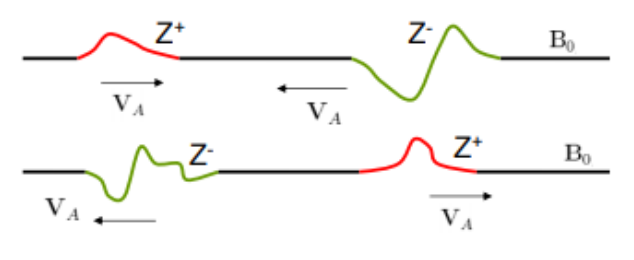
\includegraphics[width=0.7\columnwidth]{Fundamentos/InteraccionElsasser.png}
%%   \caption{Representacion esquematica de ondas de Alfvén $z^+$ y $z^−$
%%     que viajan a la velociad de Alfvén en direccion paralela y anti
%%     paralela.}
%%   \label{fig:FundInteraccionElsasser}
%% \end{figure}
%% En esta ecuación el campo magnético $\vec{B}$ se encuentra en unidades
%% de la velocidad. Utilizando estas variables, las \cref{eq2:MHDmov,
%%   eq2:MHDind} pueden reescribirse como {\color{red} CORREGIR}
%% \begin{equation}\label{eq2:MHDElsasser}
%%   \frac{\partial \vec{z^\pm}}{\partial t} + \vec{z^\pm}\cdot\nabla\vec{z^\pm} = -\nabla p_T + \nu^\pm \nabla^2\vec{z^\pm} ........
%% \end{equation}
%% donde $p_T$ es la presión total y $\nu^\pm = \frac{\nu\pm\eta}{2}$.

%% A partir de la \cref{eq2:MHDElsasser}, se pueden derivar dos de los
%% invariantes de la magnetohidrodinámica: la energía total $E$ y la
%% helicidad cruzada $H_c$:
%% {\color{red} AGREGAR}

%% Hay otro invariante presente en el modelo. La helicidad magnética
%% $H_m$ está definida como $H_m = \frac{1}{2} \int \vec{A}\cdot \vec{B}
%% dV$, donde $A$ es el potencial vector tal que $\vec{B} =
%% \nabla\times\vec{A}$. Esta cantidad permite caracterizar el flujo
%% turbulento macroscópico y permite medir topológicamente el
%% enlazamiento y anudado de las líneas de campo magnético en el plasma.

%% Como consecuencia de estas cantidades conservadas en el flujo resultan
%% algunas propiedades muy importantes en el plasma, como pueden ser que
%% la conservación de la energı́a y la helicidad magnética llevan al
%% decrecimiento colectivo y a la existencia de una cascada inversa de
%% helicidad magnética. Es decir, la helicidad fluye en sentido contrario
%% a la cascada de energı́a, desde las escalas chicas hacia la
%% macroescala.

%% La conservación de la energı́a y la helicidad cruzada resulta en lo que
%% es conocido como el alineamiento dinámico ó estado Alfvénico. Esto
%% hace que las fluctuaciones del campo magnético y el campo de
%% velocidades tiendan a tener progresivamente mayor correlación en las
%% escalas chicas.






\section{Conceptos fundamentales de turbulencia hidrodi\-námica}\label{sec:FundTurbulenciaHD}
Un flujo turbulento satisface la ecuación de Navier-Stokes
[\cite{batchelor_theory_1953}],
\begin{equation}\label{eq2:N-S}
  \frac{\partial \vec{v}}{\partial t} + \vec{v}\cdot\nabla\vec{v} =
  -\frac{1}{\rho}\nabla p + \nu\nabla^2 \vec{v},
\end{equation}
donde $\vec{v}$ es el campo de velocidades (que fluctúa en tiempo $t$
y espacio $\vec{x}$), $\nabla$ es el gradiente respecto de $\vec{x}$,
$\rho$ es la densidad, $p$ es la presión y $\nu$ es la viscosidad
cinemática. Consideraremos un fluido incompresible con densidad
constante, de modo que la ecuación de continuidad queda reducida a la
condición de divergencia nula $\nabla\cdot\vec{v} = 0$, por lo que la
presión se puede obtener mediante la condición que emerge de tomar la
divergencia de la \cref{eq2:N-S}.

El número de Reynolds macroscópico está definido como $R = vL/\nu$,
donde $v$ es la velocidad típica del fluido (la raíz cuadrática media,
$rms$, del campo de velocidades) y $L$, una escala grande típica del
problema. Este número es una medida de la importancia que
tiene el término convectivo no lineal $\vec{v}\cdot\nabla\vec{v}$
respecto del término disipativo $\nu\nabla^2 \vec{v}$ en la
\cref{eq2:N-S}.

En ausencia de viscosidad, el flujo conserva la energía cinética
global (aquí, $u^2 = \langle \left|\vec{u}\right|^2\rangle$ es el
doble de la energía por unidad de masa, donde $\langle ... \rangle$
denota promedio volumétrico). Por otra parte, cuando hay viscosidad
presente, aun para valores muy bajos, la energía decae de una forma
sumamente distintiva.


\subsection{Decaimiento global de energía}

El decaimiento global de la turbulencia incompresible, homogénea e
isotrópica fue estudiado por \cite{taylor_statistical_1935,
taylor_spectrum_1938} y por \cite{von_karman_statistical_1938},
previamente al trabajo revolucionario de
\cite{kolmogorov_local_1941,kolmogorov_decay_1941} en el rango
inercial de pequeñas escalas. La energía varía en respuesta a los
efectos viscosos de acuerdo a $dv^2/dt = -\nu
\langle\left|\nabla\times\vec{v}\right|^2\rangle$. Basándose en
resultados empíricos, Taylor encontró que el decaimiento de la energía
se comporta de acuerdo a $dv^2/dt \propto v^3$, y
\cite{von_karman_statistical_1938} proveyeron posteriormente la
primera justificación teórica de la ley de decaimiento $dv^2/dt =
-\alpha v^3/\lambda$, que ha gozado de mucho soporte empírico en
hidrodinámica.

Un elemento crucial es $\lambda$, la \textit{escala de similaridad} o
\textit{energy-containing scale}, que se comporta como $d\lambda/dt =
\beta v$. La escala de similaridad se suele asociar con la escala más
grande, o con la longitud de correlación de la turbulencia en trabajos
observacionales [\cite{batchelor_theory_1953}].  Por su parte, las
constantes $\alpha$ y $\beta$ son ambas del orden de la unidad, y
adoptan valores específicos basándose en suposiciones físicas, tales
como la permanencia de los \textit{eddies} (remolinos) de gran escala
[\cite{kolmogorov_energy-scattering_1941}], el número de Reynolds
turbulento [\cite{von_karman_concept_1949}], etc
[\cite{orszag_analytical_1970,matthaeus_anisotropic_1996}]. Esta
fenomenología de los \textit{energy-containing eddies} da una
aproximación razonable a la imagen de decaimiento global de la
energía, y clarifica cómo el reservorio de energía de grandes escalas
($\sim \lambda \sim L$) controla el proceso. Usualmente, se define el
tiempo de rotación de los remolinos (\textit{eddy turnover time}) o la
escala no lineal temporal como $\tau_{eddy} = \lambda/v$
[\cite{rose_fully_1978}], de manera que el decaimiento de la energía
ocurra a razón de $dv^2/dt = -v^2/\tau_{eddy}$. La escala temporal del
\textit{eddy turnover} es la escala fundamental de tiempo en
turbulencia, y su rol en el decaimiento global en hidrodinámica
predice el rol de las escalas de tiempo no lineales en las cascadas de
energía tanto para hidrodinámica como para MHD.

\subsection{Localidad de la transferencia de energía y espectro de Kolmogorov}

Para un fluido turbulento con alto número de Reynolds, la suposición
respecto de la tríada de interacción y el proceso de transferencia de
energía conducen hacia la famosa ley de escalas $-5/3$ de Kolmogorov
[\cite{batchelor_theory_1953, kolmogorov_local_1941}]. Brevemente,
Kolmogorov asumió que tanto la transferencia de energía como la
interacción entre escalas son locales. Para comprender esto, primero
hay que definir más o menos formalmente la energía contenida en una
escala $\ell$. Por ejemplo, la energía por unidad de masa en la escala
$\ell$ puede expresarse como
$v_\ell^2 \sim \langle |\vec{v}(\vec{x}) -
\vec{v}(\vec{x}+\vec{\ell})|^2\rangle$. Alternativamente, en el
espacio de momentos $k$, se puede computar la función de correlación
$R_{ij}(\vec{r}) = \langle\vec{v}_i(\vec{x}) \cdot
\vec{v}_j(\vec{x}+\vec{r})\rangle$, y a partir de ahí, el tensor
espectral $S_{ij}(\vec{k})$ tomando la transformada de Fourier de
$R_{ij}$. Sumando sobre todas las direcciones de $\vec{k}$ se obtiene
el espectro omnidireccional para turbulencia isotrópica, $E(k) = 4\pi
k^2 S_{ii}(k)$. Finalmente, la energía por unidad de masa asociada a
la escala $\ell \sim 1/k$ es $v_k^2 \sim \sqrt{kE(k)}$
[\cite{batchelor_theory_1953}].

Retomando, el proceso de transferencia de energía puede ser pensado de
la siguiente manera: una fuerza es aplicada a un fluido a una escala
grande $L$, inyectándole energía. El movimiento del fluido a escala
$L$ se vuelve inestable y pierde su energía en favor de sus escalas
vecinas más pequeñas, sin disiparse directamente en forma de calor
(transferencia local de energía). Este proceso se repite hasta llegar
a la escala de disipación $l_d$ (la escala de Kolmogorov), donde la
energía transferida se dispersa en forma de calor por acción
viscosa. La tasa de ingreso de energía a las escalas grande y la tasa
a la que la energía se disipa (denotada $\epsilon$) en la escala de
Kolmogorov son en promedio iguales entre sí y, en consecuencia,
iguales a la tasa de transferencia de energía a lo largo de las
escalas intermedias del espectro. El rango de escalas intermedias es
comúnmente denominado \textit{rango inercial}.

%%% Mininni
La localidad de las interacciones entre escalas parecería indicar que
las propiedades estadísticas de escalas suficientemente pequeñas
deberían ser independientes de la forma en que se generan las
turbulencias y, por lo tanto, deberían ser estadísticamente isótropas
y homogéneas, y tener un carácter universal. Esta suposición es
parcialmente cierta. Experimentos recientes mostraron desviaciones de
este comportamiento incluso para flujos hidrodinámicos simples (por
ejemplo, una recuperación de la isotropía más lenta de lo esperado o
la presencia de correlaciones a largo plazo en las escalas pequeñas
[\cite{carlier_experimental_2001, poulain_dynamics_2006,
shen_anisotropy_2000, wiltse_manipulation_1993,
wiltse_direct_1998}]). Simulaciones numéricas también dieron evidencia
de la presencia de interacciones no locales con el flujo de gran
escala, desempeñando un papel en la cascada de energía
[\cite{alexakis_imprint_2005, domaradzki_analysis_1988,
zhou_interacting_1993}]. En simulaciones numéricas con números de
Reynolds tan altos como $R_\lambda \approx 800$, se observó que el
$20\%$ del flujo de energía en las escalas pequeñas resultó de
interacciones con el flujo a gran escala
[\cite{mininni_large_2006}]. Sin embargo, simulaciones más recientes,
con números de Reynolds hasta $R_\lambda \approx 1300$ utilizando
resoluciones espaciales de $2048^3$ puntos de grilla, mostraron que a
medida que aumenta el número de Reynolds, el porcentaje de interacción
no local disminuye como una ley de potencia del número de Reynolds, lo
que sugiere que el flujo en la turbulencia hidrodinámica puede ser
predominantemente local para números muy grandes de Reynolds
[\cite{mininni_nonlocal_2008}]. Resultados teóricos más recientes lo
reafirman [\cite{aluie_scale_2010, eyink_localness_2009}], en primer
lugar mostrando que el flujo de energía en la turbulencia
hidrodinámica es local en el límite de número de Reynolds infinito, y
en segundo lugar obteniendo límites en la escala de la contribución no
local al flujo con el número de Reynolds, que están de acuerdo con los
resultados numéricos.
%%% END Mininni

De esta forma, a pesar de que los \textit{energy-containing eddies} ejercen un
control dominante sobre la tasa de transferencia energética en el
decaimiento turbulento, este control es indirecto, y las excitaciones
en el rango de \textit{energy-containing eddies} no afectan
directamente a la transferencia de energía dentro del rango
inercial. En consecuencia, la tasa promedio de disipación de energía
se identifica con la tasa de transferencia de energía espectral y con
la tasa $\epsilon$ con la que se introduce energía al sistema. Para
poder inferir la forma del espectro en el rango inercial, es necesario
estimar la magnitud de las correlaciones de la función de
transferencia (la denominada ``triple correlación'', que involucra
productos triples de las componentes de la velocidad), que son
responsables de inducir transferencia de energía. La escala temporal
del decaimiento de las correlaciones de las funciones de
transferencia, $\tau_T(k)$, puede depender de cualquier parámetro
turbulento relevante, así como también del número de onda $k$. En
términos teóricos, se podría argumentar que el flujo $\Pi(k)$ de
transferencia de energía es explícitamente proporcional a $\tau_T(k)$
y depende del número de onda y de la potencia del espectro energético
omnidireccional $E(k)$ [\cite{batchelor_theory_1953,
  monin_statistical_2013}]. En el rango inercial, como la energía es
conservada por las interacciones no lineales y se ha asumido una
cascada local, el flujo de energía $\Pi$ se vuelve independiente del
número de onda $k$ [\cite{zhou_degrees_1993,
  zhou_interacting_1993}]. Por argumentos dimensionales, se obtiene
\begin{equation}\label{eq2:transferRate}
  \epsilon = \overline{C} \tau_T(k) k^4 E^2(k),
\end{equation}
donde $\overline{C}$ es una constante del orden de la unidad.

El espectro de Kolmogorov puede recuperarse para turbulencia
estadísticamente estacionaria, homogénea e isotrópica. Para este caso,
el tiempo dinámico no lineal es
\begin{equation}\label{eq2:tauNL}
  \tau_{nl}(k) = \ell/v_k = [k^3 E(k)]^{-1/2},
\end{equation}
donde $\ell\propto 1/k$ es una escala longitudinal en el rango
inercial y $v_k = [k E(k)]^{1/2}$ es la velocidad característica de
los \textit{eddies} con número de onda $k$. Como ésta es la única
escala temporal disponible, es razonable que $\tau_T(k) =
\tau_{nl}(k)$. En consecuencia, a partir de las
\cref{eq2:transferRate,eq2:tauNL}, se encuentra que
\begin{equation}\label{eq2:Ek}
  E(k) = C_K \epsilon^{2/3} k^{-5/3},
\end{equation}
que resulta ser el espectro de Kolmogorov, observable esquemáticamente
en la \cref{fig:FundEspectroKolmogorov}. Notar que $\tau_{nl}(k) \sim
\epsilon^{-1/3} k^{-2/3}$. Aquí, $C_K$ es la constante de Kolmogorov
[\cite{sreenivasan_universality_1995, yeung_universality_1997}].
\begin{figure}[h]
  \centering
  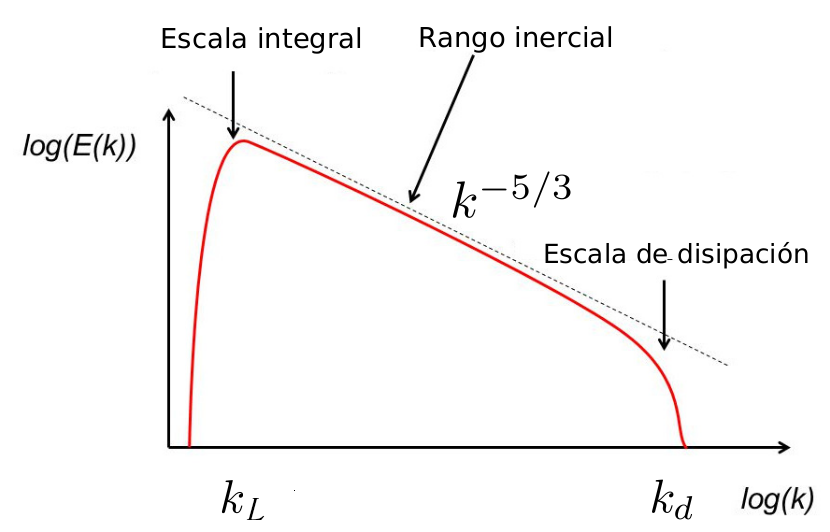
\includegraphics[width=0.7\columnwidth]{Fundamentos/EspectroKolmogorov.png}
  \caption{Representación esquemática del espectro de Kolmogorov. Se
    muestran las escalas características más importantes, la escala
    integral $k_L$ y la escala de disipación $k_d$.}
  \label{fig:FundEspectroKolmogorov}
\end{figure}


\subsection{\textit{Straining} y \textit{sweeping}}

El espectro de Kolmogorov clásico se basa en la representación de la
cascada en la cual la energía se transfiere entre escalas en forma
similar a una serie de saltos de agua, en las que cada nivel (escala)
se llena hasta derramarse en el siguiente nivel, más bajo (escala más
pequeña) [\cite{tennekes_first_1972}]. Esta cascada ocurre
principalmente como consecuencia de interacciones de \textit{eddies}
de casi el mismo tamaño (es decir, locales en el espacio de
Fourier). Estas interacciones consisten en movimientos de
\textit{straining} en los cuales un vórtice se ``estira'', produciendo
un gradiente de velocidades que distorsiona otros vórtices.


\begin{figure}[h]
  \centering
  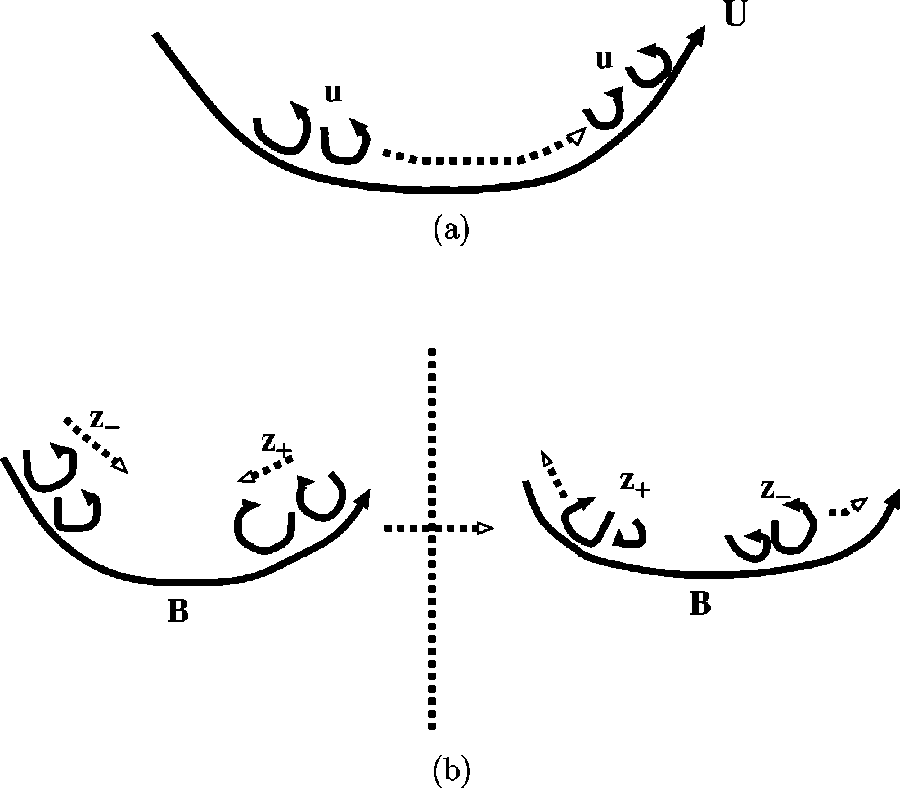
\includegraphics[width=0.7\columnwidth]{Fundamentos/fig1.png}
  \caption{Comparación entre hidrodinámica y magnetohidrodinámica: (a)
    En hidrodinámica, un flujo medio de gran escala excita
    (\emph{sweeps}) \emph{eddies} de escalas más pequeñas, sin
    afectar la transferencia de energía entre escalas
    longitudinales. (b) En magnetohidrodinámica, un campo magnético
    $\vec{B}$ de gran escala barre fluctuaciones $\vec{z}^-$ y
    $\vec{z}^+$ que se propagan en sentidos opuestos, lo cual afecta
    la transferencia de energía (ilustrado como distorsiones luego de
    que los dos tipos de fluctuaciones se hayan atravesado).}
  \label{fig:HDvsMHD}
\end{figure}



Por su parte, el flujo de gran escala arrastra los vórtices de menor
escala, pero sin inducir una distorsión apreciable en sus estructuras
dinámicas internas. La interacción directa entre las grandes escalas y
las pequeñas consiste, entonces, en un movimiento de ``barrido''
(\textit{sweeping}), que no involucra transferencia energética
significativa en el espacio de Fourier, ni cambia la forma del
espectro energético hidrodinámico. Esto se encuentra diagramado en la
figura \ref{fig:HDvsMHD}(a).

En cambio, las correlaciones temporales, o equivalentemente la forma
del espectro de frecuencias (obtenida a partir de la serie temporal de
la velocidad en un punto fijo), puede encontrarse fuertemente
influenciada por el efecto del \textit{sweeping}, dado que cualquier
fluctuación en una pequeña escala (que viene dada por movimientos de
\textit{straining}), será advectada y pasará a través del punto de
prueba, introduciendo así fuertes fluctuaciones en la serie temporal.

La aproximación de Taylor de ``turbulencia congelada'' (\textit{frozen
turbulence}, \cite{taylor_spectrum_1938}) asume que el flujo de gran
escala, con velocidad $\vec{U}$, barre la turbulencia del punto de
observación. Esta aproximación, con una velocidad constante y grande
$V$ ($\gg v$, la velocidad de las fluctuaciones), es utilizada en los
estudios en túneles de viento y en los estudios de la turbulencia en
viento solar de una única nave espacial
[\cite{jokipii_turbulence_1973}], con el objeto de poder convertir las
correlaciones temporales en espaciales. En líneas generales, la idea
es que el flujo de gran escala $V$ barre las fluctuaciones locales a
través del punto de observación más rápidamente de lo que las no
linealidades locales pueden producir distorsiones. Entonces, el
espectro de frecuencias tiene la misma forma que el de números de
onda, $E(\omega) \sim \epsilon^{2/3} V^{2/3} \omega ^{-5/3}$. El
\textit{sweeping} por flujos aleatorios (con un valor grande pero
aleatorio de $\vec{V}$) da un resultado similar
[\cite{tennekes_eulerian_1975, chen_sweeping_1989}]. En contraste,
cuando el barrido es despreciable comparado con los movimientos de
\textit{straining}, el espectro puede ser predicho por análisis
dimensional, requiriendo que la densidad espectral en frecuencias
dependa exclusivamente de la velocidad de la cascada de energía y de
la frecuencia [\cite{tennekes_eulerian_1975, nelkin_time_1990}]. Esto
implica que $E(\omega) \sim \epsilon \omega^{-2}$. De esta forma, la
presencia o ausencia de un flujo $V$ en las grandes escalas resulta
relevante para el espectro de frecuencias, si se asume la hipótesis de
\textit{sweeping}.

Por otra parte, resulta bastante claro que el \textit{sweeping} no
entra directamente en consideración en la forma que adopta el espectro
energético hidrodinámico en la \cref{eq2:Ek}
[\cite{chapman_computational_1979}]. Sin embargo, hay una relación
claramente establecida entre el \textit{sweeping} y los momentos de
orden más alto (por ejemplo, función de estructura y espectro de
energía cinética) [\cite{nelkin_time_1990}]. En particular, la
influencia que el \textit{sweeping} aleatorio ejerce en el espectro de
frecuencias puede traducirse directamente en una influencia similar en
el espectro de densidad de energía cinética (momento de cuarto orden)
[\cite{chen_sweeping_1989}]. Este resultado se condice con resultados
experimentales [\cite{van_atta_higher-order_1975,
  zhou_non-gaussian_1993}], que muestran que los espectros de momentos
de orden más alto en el rango inercial tienen los mismos exponentes en
la ley de potencias que el espectro energético, en lugar de los
valores que tendrían suponiendo sólo argumentos de \textit{straining}
puro. Estos experimentos demuestran la importancia del efecto de
barrido, la multiplicidad de escalas temporales y el rol de la no
localidad.

\subsection{Escalas temporales, cascada y clausura}

?`Cómo pueden agregarse los efectos de las escalas temporales
adicionales en una teoría simple de espectros turbulentos? Una
posibilidad es mirar con más detenimiento los conceptos físicos de la
\cref{eq2:transferRate}. Supongamos que escribimos la tasa de
transferencia espectral o el flujo de energía en la forma (mucho más
sugestiva)
\begin{equation}\label{eq2:TR_sw}
  \epsilon = \Pi(k) = \frac{u_k^2}{\tau_{sp}}.
\end{equation}
Aquí, $u_k^2$ es el doble de la energía por unidad de masa asociada a
la velocidad a escalas cercanas a $1/k$. Por compatibilidad con las
\cref{eq2:transferRate,eq2:tauNL}, podemos identificar el tiempo de
transferencia espectral de energía como $\tau_{sp}
= \tau_{nl}^2/\tau_T(k)$. En consecuencia, desarrollando diferentes
aproximaciones para el tiempo $\tau_T$ de la triple correlación, es
posible obtener una variedad de modelos para los espectros de
turbulencia.

El significado más profundo de este procedimiento simbólico puede ser
visto examinando cómo relaciones similares a las dadas por las
\cref{eq2:transferRate,eq2:TR_sw} emergen en un tratamiento
matemáticamente más formal, y cuánto más precisas se vuelven las
definiciones de las escalas temporales que entran en las teorías al
asociarlas con términos que surgen fenomenológicamente.

Una forma particularmente reveladora de la ecuación de evolución para
el espectro energético emerge de la clausura conocida como
aproximación Markoviana cuasinormal de remolinos amortiguados
(\textit{Eddy-Damped, QuasiNormal Markovian}, o \textit{EDQNM} por sus
siglas). Como una breve introducción [\cite{orszag_analytical_1970,
monin_statistical_2013, mccomb_physics_1990,
lesieur_turbulence_2008}], analicemos la parte más estructural de este
enfoque. Consideremos la ecuación de Navier-Stokes en el espacio de
momentos, $\partial_t \hat{v}(\vec{k}) = \hat{v}\hat{v} - \nu k^2
\hat{v}(\vec{k})$ [\cite{lesieur_turbulence_2008}], donde $\hat{v}$
refiere a la representación de Fourier del campo de velocidades y se
presuponen los índices cartesianos y la sumatoria sobre índices. La
ecuación para el espectro modal $E(k)/4\pi k^2 \sim \langle
\hat{v}\hat{v} \rangle$ tiene la forma
\begin{equation}\label{eq2:2ndorder}
  \left(\frac{\partial}{\partial t} + \nu k^2 \right) \langle \hat{v} \hat{v} \rangle
  = \langle \hat{v} \hat{v} \hat{v} \rangle.
\end{equation}
Esto involucra momentos de tercer orden (correlaciones triples)
$\hat{v}\hat{v}\hat{v}$, que obedecen una ecuación de la forma
\begin{equation}\label{eq2:3rdorder}
  \left(\frac{\partial}{\partial t} + \nu \left(k^2+p^2+q^2\right) \right) \langle \hat{v}(\vec{k}) \hat{v}(\vec{p}) \hat{v}(\vec{q}) \rangle = \langle \hat{v} \hat{v} \hat{v} \hat{v} \rangle,
\end{equation}
donde $\vec{k}$, $\vec{p}$ y $\vec{q}$ denotan vectores de onda. El
``problema de clausura'' se refiere a la ocurrencia de correlaciones
de cuarto orden en las ecuaciones para la correlación de tercer orden,
correlaciones de quinto orden en las ecuaciones para cuarto orden, y
así sucesivamente, no siendo posible clausurar el problema a ningún
orden. Los métodos de clausura adoptan aproximaciones para momentos de
orden más alto en términos de momentos de órdenes más bajos. La
aproximación cuasinormal (QNA, \cite{millionshchikov_1941}) representa
el momento de cuarto orden de la \cref{eq2:3rdorder} como una suma
sobre productos de momentos de segundo orden. Esto permite encontrar
una solución para los momentos de tercer orden, que se pueden
sustituir entonces en la \cref{eq2:2ndorder}, dando lugar a un sistema
de ecuaciones cerrado para los momentos de segundo orden, y en
consecuencia para el espectro de
energía. \cite{orszag_analytical_1970} y otros introdujeron
refinamientos adicionales y aproximaciones que dan lugar a la
aproximación \textit{EDQNM}. Este es en muchos aspectos un modelo
aceptable para turbulencia, y conduce a una ecuación para el espectro,
que puede ser escrita como
\begin{equation}\label{eq2:spectrumeq}
  \left( \frac{\partial}{\partial t} + \nu k^2 \right) E(k, t) = \int\int_\Delta dp dq \Theta_{kpq} E(q,t) \times \left[ A(k, p, q) E(q, t) - B(k, p, q) E(k, t)\right].
\end{equation}

Aquí, las integrales son sobre todos los vectores de onda con la
restricción $\vec{q} = \vec{k} - \vec{p}$, y $A$ y $B$ son
coeficientes de acoplamiento con unidades de número de onda.  El
tiempo $\Theta_{kpq}$ aparece como un tiempo característico de
relajación debido a las transferencias no lineales y a la viscosidad
de $\langle \hat{v}(\vec{k}) \hat{v}(\vec{p}) \hat{v}(\vec{q})
\rangle$.  El flujo de energía en el rango inercial puede ser
calculado a partir de la integral $\Pi(k) = -\frac{\partial}{\partial
  t} \int_0^k E(k, t) dk$, utilizando la expresión \textit{EDQNM} en
el miembro derecho de la \cref{eq2:spectrumeq}. Finalmente, estimando
que las contribuciones dominantes provienen de $p \approx q \approx
k$, se llega a $\epsilon = \Pi(k) = \tau_T(k) k^4 E^2(k)$, previamente
obtenido por análisis dimensional en el rango inercial. Cabe notar que
el ``tiempo de decaimiento triple'' $\tau_T(k)$, que anteriormente
asumimos que aparecía por argumentos heurísticos, es ahora
identificable con \textit{eddy-damping time} $\Theta_{kkk}$ (o
``tiempo de amortiguación de los remolinos'') que emerge como el
tiempo clave en la evaluación del flujo de energía
\textit{EDQNM}. Este resultado nos da confianza, porque ahora el
resultado del análisis dimensional adquiere un contexto dentro de la teoría
analítica. Sin embargo, es muy importante tener en cuenta que el rol
físico que cumple la tasa de amortiguamiento de los \textit{eddies} en
la correlación triple es el de restaurar, de una forma aproximada, el
efecto de descorrelación de los cumulantes de tercer orden, que
habíamos despreciado en la QNA. En efecto, la elección del
\textit{eddy-damping rate} conlleva que la aproximación \textit{EDQNM}
tenga una ley espectral particular. De esta forma, a pesar de la
elegancia algebraica, la clausura \textit{EDQNM} requiere que
entendamos correctamente la física que determina el tiempo de
descorrelación. Aún así, la identificación $\tau_T(k) = \Theta_{kkk}$
nos da confianza respecto de cómo tales escalas de tiempo actúan en
teorías más formales, mientras que nos da una cadena de razonamiento
que conecta el análisis dimensional con la estructura matemática de la
turbulencia. Este es un marco útil cuando extendemos el uso de las
cascadas fenomenológicas para incluir otras escalas de tiempo (y sus
efectos) en MHD.

Otra teoría de clausura, la Aproximación de Interacción Directa de
Kraichnan (\textit{DIA}, por sus siglas en inglés, 1957), quizás el
arquetipo de teorías de clausura estadísticas de turbulencia, procede
a través de una expansión de perturbaciones en las que el orden más
bajo de la velocidad obedece exactamente la estadística gaussiana. La
\textit{DIA} busca una solución al problema de clausura en turbulencia
expandiendo en un parámetro $\delta$, permitiendo que los términos no
lineales en la ecuación de evolución sean del orden de $\delta$, que
eventualmente se igualará a la unidad. Para facilitar la solución, se
define un propagador (una función de Green) $\tilde{G}(\vec{k}, t,
t')$, el cual representa la respuesta del sistema a una función
gaussiana de forzado del sistema correlacionada con $\delta$. Un punto
clave es obtener las ecuaciones acopladas de renormalización para el
propagador promediado $G = \langle\tilde{G}\rangle$ y para la función
espectral retrasada $Q(\vec{k}, t, t')$, que determina cuán
rápidamente las correlaciones decaen en el tiempo. Cabe mencionar que
la correlación de dos puntos espacio-temporales puede definirse como
$R_{ij}(\vec{r}, \tau) = \langle v_i(\vec{x}, t) v_j(\vec{x}+\vec{r},
t+\tau)\rangle$, mientras que el tensor espectral retrasado en el
tiempo $S_{ij}(\vec{k},\tau)$ es la transformada de Fourier espacial,
con la componente temporal (el retraso temporal) ahora denotando la
descorrelación temporal de ambos elementos del espectro. La función
espectral $Q$ de DIA es, esencialmente, la traza de $S$.

Mientras los detalles no son importantes para el presente escrito
(para más detalles, ver
\cite{leslie_developments_1973, mccomb_physics_1990}), la solución
simultánea para $Q$ y $G$ establece la naturaleza de dos tiempos de
descorrelación en cada número de onda. Acordemente, en el formalismo
del propagador, la dependencia temporal de las correlaciones de tercer
orden se encuentra establecida en términos de las correlaciones de
segundo orden.

En general, los modelos de \textit{EDQNM} y \textit{DIA} son bastante
distintos, pero \cite{mccomb_physics_1990} argumenta que hay una
interesante modificación \textit{ad hoc} a \textit{DIA} que muestra
una conexión estructural entre ambos modelos. Supongamos que en lugar
de resolver las ecuaciones isotrópicas de \textit{DIA} para $Q$ y $G$
de la forma usual, empezamos con \textit{DIA} y hacemos la simple
aproximación, para $t>t'$, $Q(\vec{k}, t, t') = S(\vec{k}, t')
e^{-\gamma(k) (t-t')}$ y $G(\vec{k}, t, t') = e^{-\gamma(k)(t-t')}$,
donde la tasa de descorrelación es tomada para ser el recíproco del
tiempo no lineal, $\gamma(k) = 1/\tau_{nl}(k) \sim \epsilon^{1/3}
k^{2/3}$. En este caso, esta ecuación ``pseudo - \textit{DIA}'' para
la evolución espectral se vuelve idéntica a la ecuación espectral de
\textit{EDQNM}, la \cref{eq2:spectrumeq}. Esta identificación no debe
ser tomada muy seriamente, ya que \textit{DIA} prescribe el tiempo de
descorrelación a su manera. Sin embargo, en la medida en que el límite
de McComb es realizable, la aproximación \textit{EDQNM}, la
\textit{DIA} modificada y el enfoque fenomenológico concuerdan: la ley
espectral de potencias viene determinada por la elección de la escala
temporal $\Theta_{kpq}$. Entonces, resulta razonable buscar un
tratamiento fenomenológico del espectro MHD para entender la variedad
de conclusiones que pueden ser aplicables al espacio y a plasmas
astrofísicos.




\section{Turbulencia magnetohidrodinámica}\label{sec:FundTurbulenciaMHD}

Habiendo hecho un análisis básico de cómo las diferentes escalas
temporales aparecen en el caso de turbulencia hidrodinámica, veamos
ahora el caso magnetohidrodinámico, en el cual, si bien es más
complejo, es posible aplicar algunas de las ideas para entender qué
espectros son esperables.

\subsection{Ecuaciones MHD y conceptos físicos básicos}

Un plasma, descripto como un fluido eléctricamente conductor,
evoluciona en respuesta a fuerzas tanto mecánicas como
electromagnéticas. Por simplicidad, nos focalizaremos en el modelo
incompresible con densidad constante, que provee un contexto adecuado
para muchos de los problemas de turbulencia MHD
[\cite{biskamp_magnetohydrodynamic_2003}]. El modelo MHD incompresible,
en términos de la velocidad $\vec{v}$ del fluido y del campo magnético
$\vec{B}$, consta de una ecuación de momentos
\begin{equation}\label{eq2:NS-MHDv}
  \frac{\partial \vec{v}}{\partial t} + \vec{v} \cdot \nabla\vec{v} = -\frac{1}{\rho} \nabla p + \frac{1}{4\pi\rho} \left(\nabla\times\vec{B}\right)\times\vec{B} + \nu \nabla^2 v,
\end{equation}
y de una ecuación de inducción magnética
\begin{equation}\label{eq2:NS-MHDB}
  \frac{\partial \vec{B}}{\partial t} = \nabla \times \left(\vec{v}\times\vec{B}\right) + \mu \nabla^2 \vec{B}.
\end{equation}
La densidad del plasma $\rho$, la viscosidad cinemática $\nu$ y la
difusividad magnética $\mu$ se consideran uniformemente constantes. La
velocidad y el campo magnético son solenoidales, $\nabla\cdot\vec{v}
= \nabla\cdot\vec{B} = 0$, y la presión $p$ está determinada por la
divergencia de la \cref{eq2:NS-MHDv}. Los números de Reynolds cinético
$R = vL/\nu$ y magnético $R_m = vL/\mu$ (aquí, $v$ es una velocidad
típica y $L$ es una escala espacial típica) miden el peso relativo
entre los términos no lineales y los términos lineales disipativos en
las ecuaciones dinámicas. Se tiene MHD altamente turbulento cuando los
valores de $R$ y $R_m$ suficientemente altos.

Antes de continuar, recordemos que el modelo MHD es frecuentemente
aplicado al espacio y a plasmas astrofísicos. No obstante, en ninguno
de estos casos suele ser clara la derivación del modelo. Para plasmas
poco colisionales, la estructura básica de MHD emerge por las
conservaciones de la masa, el momento y la energía, junto con las
leyes de Maxwell-Ampère y Faraday, e ignorando las corrientes de
desplazamiento y adoptando una forma adecuada de la ley de Ohm. Aún
así, para la mayoría de las aplicaciones no hay un camino claro para
cerrar el sistema con un único campo de presiones isótropo, ni hay
cálculos convincentes para la viscosidad, la resistividad, y otros
coeficientes de transporte como la conductividad térmica.

Un camino posible para trabajos numéricos es adoptar coeficientes
disipativos escalares, eligiendo los valores de acuerdo a las
limitaciones numéricas de resolución espacial, más que en el realismo
físico. Para MHD turbulento esto puede estar justificado asumiendo que
la cascada no lineal se da principalmente desde las escalas grandes a
las pequeñas, y el papel específico de la disipación mecánica es el de
absorber cualquier energía que llegue a escalas pequeñas vía
transferencia espectral. Esto es parcialmente satisfactorio, y sería
deseable una mayor comprensión teórica de la naturaleza de la
disipación en las aplicaciones de MHD poco colisional, aunque puede no
ser simple ni tener una forma universal. Por el lado positivo, cuando
se tienen observaciones experimentales disponibles, como es en el caso
del viento solar, se puede ver que el rango inercial es amplio, por lo
que el rango de inyección de energía se encuentra bien separado en
escala del rango disipativo, donde el espectro se vuelve más empinado
[\cite{leamon_observational_1998}]. Con esta base, es posible inferir
un Reynolds efectivo para el viento solar, y por analogía para
cualquier plasma turbulento cuyo rango inercial sea conocido. Por
ejemplo, ignorando las diferencias entre la disipación viscosa y
resistiva, uno podría emplear una estimación hidrodinámica para el
número de onda disipativo, $k_d
= \left(\epsilon/\nu^3\right)^{1/4}$. Usando la estimación de
Taylor-von Karman de la tasa de decaimiento $\epsilon = v^3/\lambda$,
puede escribirse $k_d \lambda = R^{3/4}$, o $R =
\left(k_d \lambda\right)^{4/3}$, donde $R$ es el número de
Reynolds. La cantidad $k_d \lambda$ es aproximadamente el ancho de
banda del rango inercial. De esta forma, para un rango inercial de
tres a cuatro décadas (por ejemplo, el viento solar), uno tiene $R
\approx 10^5$. Para la corona solar, se estima un rango inercial de
cinco a seis décadas, por lo que $R \approx 10^8$. En general, cuando
hay un rango inercial de varias décadas, uno puede inferir que el
Reynolds efectivo para las grandes escalas es un número grande, aún
cuando no se tenga una formulación teórica del mecanismo de
disipación.

El campo magnético puede contener una parte uniforme $\vec{B}_0$
(campo magnético DC) o que varía muy suavemente (identificable con el
campo magnético medio local), más fluctuaciones de pequeña escala
$\vec{b}$; es decir, $\vec{B} = \vec{B}_0 + \vec{b}$. El campo
magnético de gran escala permite y respalda la propagación de ondas
hidromagnéticas (ondas de Alfv\'en). Estas ondas son fluctuaciones
transversales al campo magnético medio, propagándose en la dirección
de campo magnético medio a la velocidad de Alfv\'en $V_A =
B_0/\sqrt{4\pi\rho}$, y siguiendo la relación de dispersión $\omega
= \pm V_A k_\parallel$, con $k_\parallel$ la dirección paralela al
campo medio $\vec{B_0}$, obtenida a partir de la linealización de
las \cref{eq2:NS-MHDv,eq2:NS-MHDB}.

Aún el caso más simple de MHD, asumiendo incompresibilidad, isotropía,
estacionariedad y homogeneidad, es más complejo que el caso
hidrodinámico. Hay dos campos distintos con los que hay que lidiar, el
magnético y el de velocidades, y se agrega complejidad debido al
efecto de la propagación de ondas de Alfv\'en. De esta forma, hay al
menos dos clases de escalas temporales involucradas, el tiempo no
lineal y el tiempo de Alfv\'en (el tiempo para que una fluctuación se
propague dada una escala espacial). Es más, el campo magnético de gran
escala introduce una dirección preferencial, y los efectos
anisotrópicos que esto genera se hacen presentes en las fluctuaciones.

Aquí hemos arribado a una gran diferencia entre turbulencias
hidrodinámica y magnetohidrodinámica. A diferencia del caso
hidrodinámico, el efecto no local de las escalas grandes sobre las
pequeñas, el \textit{sweeping}, tiene un papel importante en
turbulencia MHD, pues el campo magnético medio no puede ser
removido por una transformación de Galileo. De hecho, comenzando por
\cite{iroshnikov_turbulence_1964} y
\cite{kraichnan_inertial-range_1965}, hay argumentos para plantear que
el \textit{sweeping} juega un papel importante aún en el caso de
ausencia de campo magnético DC. Además, si hay un campo magnético de
gran escala, las fluctuaciones de pequeña escala sufren un efecto
similar al \textit{sweeping} debido a la propagación de ondas de
Alfv\'en (\textit{sweeping} magnético). Es más, la presencia de un
campo magnético permite la existencia de otro tiempo característico,
que competirá con el tiempo no lineal y el de \textit{sweeping}.

Para discutir esto, resulta más sencillo escribir las ecuaciones MHD
en una forma más simétrica, utilizando los denominados campos de
Els\"asser [\cite{elsasser_hydromagnetism_1956}], $\vec{z}^\pm =
\vec{v} \pm \vec{b}/\sqrt{4\pi\rho}$,
\begin{equation}\label{eq2:MHDElsasser}
  \frac{\partial \vec{z}^\pm}{\partial t} \mp \vec{V_A} \cdot \nabla\vec{z}^\pm = -\vec{z}^\mp \cdot \nabla\vec{z}^\pm - \frac{1}{\rho} \nabla P + \mu \nabla^2 \vec{z}^\pm,
\end{equation}
donde hemos explícitamente separado el término que involucra el campo
magnético de gran escala (escrito en términos de la velocidad de
Alfv\'en $\vec{V_A}$). Por simplicidad, hemos asumido $\nu = \mu$. La
presión total $P = p + B^2/8\pi$ actúa de manera de hacer cumplir la
condición $\nabla\cdot\vec{z}^\pm = 0$.

Eligiendo o bien $\vec{z}^+ = 0$ o bien $\vec{z}^- = 0$, obtenemos las
soluciones exactas de las ecuaciones MHD ideales (sin disipación). El
campo no nulo normalmente se dice que corresponde a paquetes de onda
que se propagan a lo largo de la dirección de campo medio. Esta
descripción puede ser confusa, pues los ``paquetes'' pueden no estar
localizados ni propagándose. Las fluctuaciones no propagantes con
vectores de onda perpendiculares a la dirección del campo magnético
medio tienen velocidad de fase nula. En cualquier caso, ambos tipos de
fluctuaciones $\vec{z}^\pm$ son necesarias para que los términos no
lineales sean no nulos y haya turbulencia. Este hecho fue apuntado por
\cite{kraichnan_inertial-range_1965}, y discutido en el contexto de
aplicaciones en física espacial [\cite{dobrowolny_fully_1980}] y en
los modelos de calentamiento de la corona solar
[\cite{dmitruk_conditions_2001}].

\cite{kraichnan_inertial-range_1965} señaló que el campo
magnético medio barre las estructuras a pequeña escala con las que
interactúa, y durante ese momento se produce una transferencia no
lineal de energía entre distintas escalas longitudinales (en la
representación de Kraichnan, los paquetes de onda sufren breves
``colisiones'' durante las cuales ocurre transferencia de
energía). Esto se ilustra en la figura \ref{fig:HDvsMHD}(b). De esta
manera, las escalas pequeñas interactúan no sólo a través de los
\textit{eddies}, sino también a través de los paquetes Alfv\'en, que
reducen el flujo de energía a escalas pequeñas al aumentar su tiempo
de transferencia [\cite{chen_inhibition_1997}]. Esto introduce en la
práctica una interacción no local a medida que las ondas se propagan a
lo largo del campo a gran escala [\cite{gomez_validity_1999}].



Para flujos turbulentos MHD con un número de Reynolds alto, en
entornos astrofísicos y espaciales, existe una separación de escala
entre distintos procesos físicos a grandes y pequeñas
escalas. Específicamente, se divide la dinámica en una parte de
pequeña escala, que contiene acoplamientos de escalas
``pequeña-pequeña'' y ``pequeña-grande'', y en otra parte, de gran
escala [\cite{zhou_transport_1990}]. Cuando los campos de pequeña
escala ocupan un amplio ancho del espectro, se tiende a tratar el
acoplamiento de escalas ``pequeña-pequeña'' como turbulento,
involucrando acoplamientos que son principalmente locales en el
espacio de escalas.

El estudio de turbulencia MHD en los contextos espaciales y
astrofísicos a menudo se vuelven manejables cuando se introduce alguna
forma de separación de escala. En la aproximación más simple, una
pequeña parte de un sistema MHD no homogéneo podría tratarse como
``localmente homogéneo''. La turbulencia en el viento solar es un
ejemplo posible, en el que adicionalmente hay muchas mediciones que
hacen posible la corroboración teórica a partir de observaciones
[\cite{tu_mhd_1995, goldstein_magnetohydrodynamic_1995}]. Los primeros
estudios observacionales [\cite{coleman_turbulence_1968}] encontraron
que las fluctuaciones temporales de la velocidad del plasma, desde el
punto de referencia de una nave espacial, admiten una ley de potencias
para el espectro de escalas, un reminiscente de la descripción de
Kolmogorov de la turbulencia de un fluido no cargado. Las
observaciones también revelaron una correlación distintiva entre la
velocidad y el campo magnético, que sugiere la presencia de ondas de
Alfv\'en \textit{outward-traveling} de gran amplitud
[\cite{coleman_turbulence_1968, belcher_large-amplitude_1971,
jokipii_turbulence_1973}].

El viento solar, como la mayoría de los sistemas astrofísicos reales
en los que se encuentra turbulencia, es compresible e inhomogéneo a
grandes escalas. Las inhomogeneidades de gran escala, como cizallas de
velocidad o gradientes de temperatura y densidad, pueden suministrar
energía a la turbulencia de pequeña escala. En el viento solar, las
fluctuaciones observadas se dan en todas las escalas, con escalas de
correlación ($\lambda \sim 0.02$AU en la órbita terrestre) mucho más
pequeñas que la escala del sistema ($1$AU o más). El rango inercial de
la turbulencia MHD se extiende desde $\lambda$ hasta escalas 1000
veces más chicas, cercanas a la giroescala térmica de los
iones. Entonces, la actividad turbulenta de interés está bien
separada, en escalas de longitud, de las inhomogeneidades de gran
escala del viento solar. Es más, las propiedades de gran escala, tales
como el flujo medio y el campo magnético medio, son relativamente
coherentes y reproducibles. Entonces, el viento solar suele ser
descripto en términos del flujo canónico promedio y de propiedades del
campo magnético, tales como viento tranquilo de baja velocidad a bajas
latitudes; viento caliente, menos denso y más rápido a altas
latitudes; una espiral de Arquímedes, y otras idealizaciones con
características de gran escala. Aún cuando están presentes estructuras
dinámicas de gran escala, estas características pueden verse con
cierto grado de reproducibilidad.

En contraste, las fluctuaciones del campo observables en las pequeñas
escalas del viento solar, suelen verse como aleatorias y localmente
homogéneas. Estas fluctuaciones fueron tratadas originalmente
utilizando MHD linealizado débilmente inhomogéneo (teoría WKB)
[\cite{parker_dynamical_1965, hollweg_alfven_1973,
  hollweg_transverse_1974, hollweg_transition_1986,
  jacques_momentum_1977, matthaeus_transport_1994}], que describe la
propagación de fluctuaciones Alfv\'enicas de onda corta en un flujo
inhomogéneo. La presente perspectiva es que el medio es localmente
incompresible [\cite{matthaeus_evidence_1990}] y es descripto
aceptablemente como turbulencia MHD.

La dicotomía entre la representación de ``turbulencia'' no lineal y la
representación de ``ondas'' lineales se empapa de 40 años de estudio
del viento solar y espeja el tema básico de la presente tesis: las
características observables de la turbulencia MHD emergen de un
balance entre la propagación de ondas y el \textit{sweeping}
aleatorio, por un lado, y las distorsiones o \textit{strainings}, por
otro.


\subsection{Fenomenología del decaimiento MHD}
Mientras en turbulencia hidrodinámica lidiamos con una única densidad
de energía $v^2$ y un único tensor de correlación de dos puntos
asociado, la presencia de dos campos dinámicos en MHD introduce cuatro
tipos de correlaciones o energías (por unidad de masa): la energía
cinética $E_v = \langle \left| \vec{v}\right|^2\rangle/2$, la energía
magnética $E_b = \langle \left| \vec{b}\right|^2\rangle/2$, la
helicidad cruzada $H_c = \langle \vec{v} \cdot \vec{b} \rangle =
\langle \left| \vec{z}^+\right|^2 - \left| \vec{z}^-\right|^2
\rangle/4$ y la diferencia de energías $D = \langle \left|
\vec{v}\right|^2 - \left| \vec{b} \right|^2 \rangle/2 = \langle
\vec{z}^+ \cdot \vec{z}^- \rangle/2$. (Se utilizan unidades de
velocidad de Alfvén, en la que el campo magnético $\vec{b} \rightarrow
\vec{b}/\sqrt{4\pi\rho}$ tiene dimensiones de velocidad.) Notar que la
helicidad cruzada es la diferencia de las energías de Els\"asser
$Z_\pm^2 = \langle \left| \vec{z}^\pm \right|^2 \rangle/4$. La
situación más simétrica se da cuando se tiene equipartición, $D = 0$ y
$H_c = 0$. Para este caso, ni los campos magnético y de velocidades,
ni las variables de Els\"asser, se encuentran correlacionadas entre
sí. En este tipo de MHD, $Z_-^2 = Z_+^2 = Z^2$, y una simple extensión
de la fenomenología del decaimiento hidrodinámico funciona bien para
MHD con un número de Reynolds moderado
[\cite{hossain_phenomenology_1995}]. En particular, $dZ^2/dt = -\alpha
Z^3/\lambda$ y $d\lambda/dt = \beta Z$, donde $\alpha$ y $\beta$ son
constantes de orden uno y $\lambda$, una escala de similaridad. La
elección de las constantes puede tener una interpretación física como
en el caso hidrodinámico [\cite{matthaeus_anisotropic_1996}]. Este
enfoque de tipo hidrodinámico para el decaimiento MHD se ha utilizado
en el modelado del transporte de la turbulencia en el viento solar;
dicho modelo proporciona una explicación razonablemente precisa del
perfil radial de la turbulencia del viento solar, desde la órbita
terrestre ($1$AU) hasta más de $60$AU [\cite{smith_heating_2001}].

Más generalmente, no podemos asumir helicidad cruzada nula, y la
fenomenología del decaimiento deberá tener en consideración la
asimetría entre $Z_+^2$ y $Z_-^2$. Esta situación introduce escalas de
tiempo adicionales. Las bases de esto se encuentran, por ejemplo, en
las discusiones fenomenológicas de \cite{iroshnikov_turbulence_1964},
\cite{kraichnan_inertial-range_1965} y \cite{dobrowolny_fully_1980}, y
en el tratamiento detallado de clausuras MHD por
\cite{pouquet_strong_1976} y \cite{grappin_dependence_1983}. La
aproximación fenomenológica propuesta por
\cite{hossain_phenomenology_1995} plantea que
\begin{equation}
  \frac{dZ_\pm^2}{dt} = -\alpha_\pm \frac{Z_\pm^2}{\tau_{sp}^\pm}
\end{equation}
en términos de las constantes $\alpha_+$ y $\alpha_-$, de forma
similar a lo ya expuesto para el caso hidrodinámico. La estimación más
simple [\cite{pouquet_strong_1976, grappin_dependence_1983}] es que el
tiempo de transferencia espectral se identifique con el tiempo del
\textit{eddy turnover} (tiempo no lineal), es decir, $\tau_{sp}^\pm =
\tau_{nl}^\pm$; este último, teniendo en cuenta la naturaleza de las
interacciones entre $\vec{z}^+$ y $\vec{z}^-$, puede ser estimado como
$\tau_{nl}^\pm = \lambda_\pm / Z_\mp$ para escalas de similaridad
$\lambda_\pm$. Para esta elección, la ecuación de decaimiento de la
energía se puede escribir como
\begin{equation}\label{eq2:elsasserdecay}
  \frac{dZ_\pm^2}{dt} = -\alpha_\pm \frac{Z_\pm^2 Z_\mp}{\lambda_\pm}
\end{equation}

Para cerrar el sistema de ecuaciones del decaimiento, se debería
elegir (y verificar si es posible) una ecuación de evolución para las
escalas de similaridad $\lambda_\pm$. Una posibilidad es
$d\lambda_\pm/dt = \beta_\pm (Z_+Z_-)^{1/2}$
[\cite{hossain_phenomenology_1995}], pero se mantiene cierta dificultad
en verificar el comportamiento de las escalas de similaridad, puesto
que deben resolverse (en, por ejemplo, las simulaciones), tanto las
escalas más pequeñas (de manera de resolver adecuadamente la cascada
directa de energía) como las escalas más grandes.

Otra dificultad con el análisis del decaimiento MHD fenomenológico es el grado de
certeza y generalidad con el que se hace la identificación
$\tau_{sp}^\pm \rightarrow \tau_{nl}^\pm$, utilizada en la
\cref{eq2:elsasserdecay}. Efectivamente, cabe preguntarse si hay alguna
otra escala temporal que entre en juego en el decaimiento global, por
ejemplo, algún otro tipo de escala tipo \textit{sweeping} que pueda
descorrelacionar las interacciones de las grandes escalas no lineales,
modificando así la tasa global de decaimiento de energía. Dichas
cuestiones serán discutidas a continuación, en el contexto del rango
inercial de la turbulencia MHD, para los casos tanto isotrópico como
anisotrópico de MHD, éste último con la presencia de un campo
magnético de gran escala.

Sin embargo, para el rango de escalas energéticas, ese problema
continúa ambiguo. Para turbulencia homogénea
periódica, \cite{hossain_solar_1996} plantearon que el desarrollo de
una anisotropía relativa a un campo magnético de gran escala actúa
saturando y minimizando el efecto de descorrelación en el rango de
escalas energéticas. Sin embargo, esto presupone que el tiempo de
Alfv\'en de gran escala $\tau_A = \lambda/V_A$ es no demasiado
pequeño. Esto puede depender de las condiciones iniciales, tanto como
de las condiciones de contorno. Un tema particularmente sensible en
las aplicaciones [\cite{dmitruk_conditions_2001}] es si las
condiciones de contorno permiten la persistencia de estructuras no
propagantes, tales como turbulencia 2D, que no son afectadas por el
tiempo de barrido debido a ondas de Alfv\'en, $\tau_A$. Además, las
interacciones entre condiciones de contorno, efectos de propagación de
ondas, e interacciones no lineales, pueden tener un impacto en el
nivel de turbulencia (medido como tasa transferencial de energía)
mantenido por el sistema (\cite{dmitruk_lowfrequency_2003} para
aplicación en modelo de calentamiento coronal). Por ahora, sin
embargo, notamos que la multiplicidad de escalas temporales en MHD
puede afectar también la dinámica del rango de energías. En esos
casos, los detalles del problema específico pueden influir en el
tiempo de decaimiento energético. Para ciertos problemas estándar,
tales como MHD periódica u homogénea con condiciones
\textit{band-limited} iniciales (excitación de modos en ciertas
escalas limitadas), hay evidencia numérica que apoya la afirmación de
que el tiempo de decaimiento global está asociado mayoritariamente con
efectos no lineales, y que los efectos de los tiempos de sweeping y de
Alfv\'en no son significativos. Claramente, esta conclusión
necesitaría ponerse a prueba en otros problemas. Por ejemplo, el caso
de fluctuaciones de Els\"asser espacialmente localizadas, bajo la
influencia de un campo magnético DC [\cite{parker_cosmical_2019}]
podría presentar un contraste interesante al caso de turbulencia
homogénea. Con este trasfondo, veamos ahora el rol de escalas
temporales en las varias posibles cascadas MHD en el rango inercial.


\subsection{MHD isótropo}
\subsubsection{Cuando el \textit{straining} local es dominante: escaleo de Kolmogorov}

\cite{fyfe_high-beta_1976} han sugerido que el razonamiento original
de Kolmogorov y el espectro $k^{-5/3}$ asociado son aplicables a
MHD. La suposición implícita es que el tiempo no lineal de distorsión
de \textit{eddies} es más rápido que el asociado a propagación de
ondas. Esto implica que la escala de tiempo relevante es $\tau_{nl}$ y
que el \textit{straining} domina sobre el
\textit{sweeping} aleatorio y la propagación de ondas. Este enfoque
parece razonable cuando la helicidad cruzada es pequeña, los campos
magnético y de velocidades se encuentran cercanos a equipartición, y
el campo magnético de grandes escalas no es demasiado grande.

\begin{figure}[h]
  \centering
  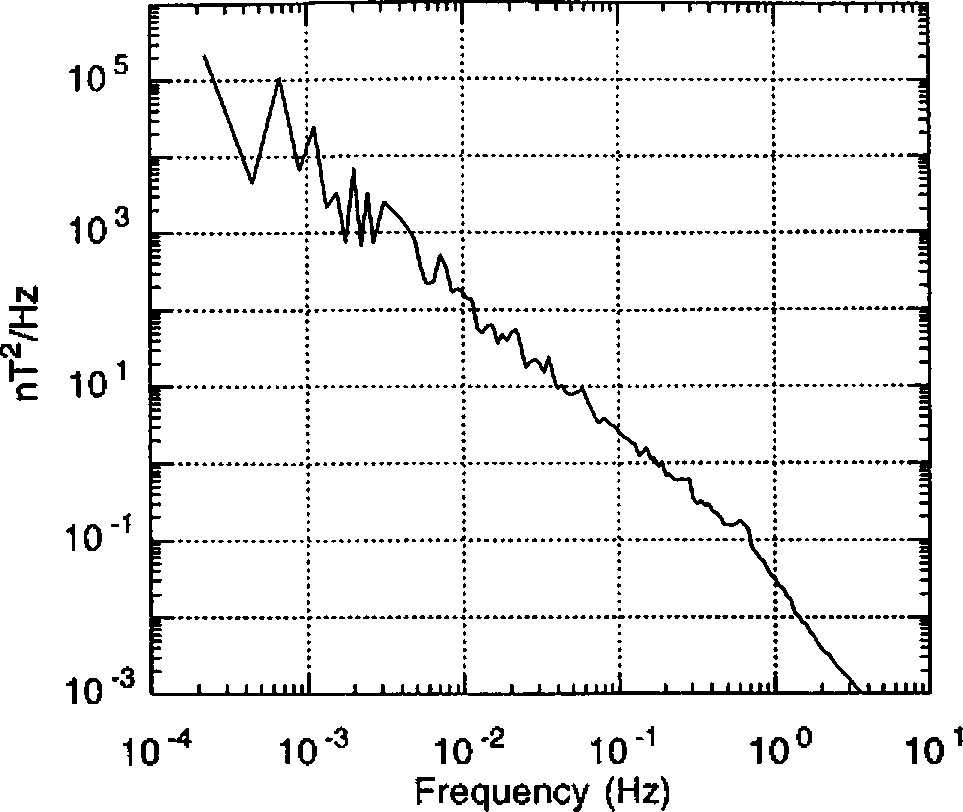
\includegraphics[width=0.7\columnwidth]{Fundamentos/fig2.png}
  \caption{Traza de la matriz espectral de potencias del campo
    magnético, medido por el magnetómetro Mariner 10 en 1974. Los
    resultados muestran que el espectro del viento solar escala con la
    pendiente $-5/3$ de Kolmogorov. Adaptado de
    \cite{goldstein_magnetohydrodynamic_1995}.}
  \label{fig:experimentalcascade}
\end{figure}

Una de las fuentes más importantes de apoyo para el escaleo $k^{-5/3}$
en MHD proviene de las observaciones \textit{in situ} del viento solar
hechas por naves espaciales, en las que ese escaleo suele ser
estadísticamente distinguible de otras leyes de potencia
propuestas. Un ejemplo se observa en la figura
\ref{fig:experimentalcascade}. Típicamente, el espectro energético
magnético $E_b(k)$ muestra una ley de potencias similar a $k^{-5/3}$ a
lo largo de tres décadas en número de
onda. \cite{matthaeus_measurement_1982} reportaron dicha ley de
potencias entre $10^{-11}/cm^{-1}$ y $3\times 10^{-9}/cm^{-1}$, con un
índice espectral de $-1.73\pm0.08$. La descomposición espectral de la
energía total, $E(k) = E_b(k) + E_u(k)$, también muestra típicamente
una ley de potencias, y hay casi equipartición entre la energía
cinética y magnética en el rango inercial. Para el total de la
energía, Matthaeus y Goldstein reportaron una dependencia de la forma
$E(k)\sim k^{-1.69\pm0.08}$ en todo el rango, salvo en los números de
onda más bajos. La expectación de equipartición en las escalas del
rango inercial es conocida como \textit{efecto de Alfv\'en}
[\cite{kraichnan_inertial-range_1965}]. La ocurrencia frecuente de
fluctuaciones Alfv\'enicas en la heliosfera interna es indicativo no
sólo de una cuasi equipartición energética, sino también de la
presencia de helicidad cruzada (\cref{fig:equiparticion})
[\cite{coleman_turbulence_1968, dobrowolny_fully_1980,
grappin_alfvenic_1982, grappin_dependence_1983,
pouquet_growth_1986}]. Generalizando, el viento solar evoluciona en la
heliosfera externa hacia estados menos Alfv\'enicos, pero permanece
casi equiparticionado entre las energías cinética y magnética
[\cite{roberts_origin_1987, roberts_amplitudes_1990}], y generalmente
$1<E_v(k)/E_b(k)<2$.

\begin{figure}[h]
  \centering
  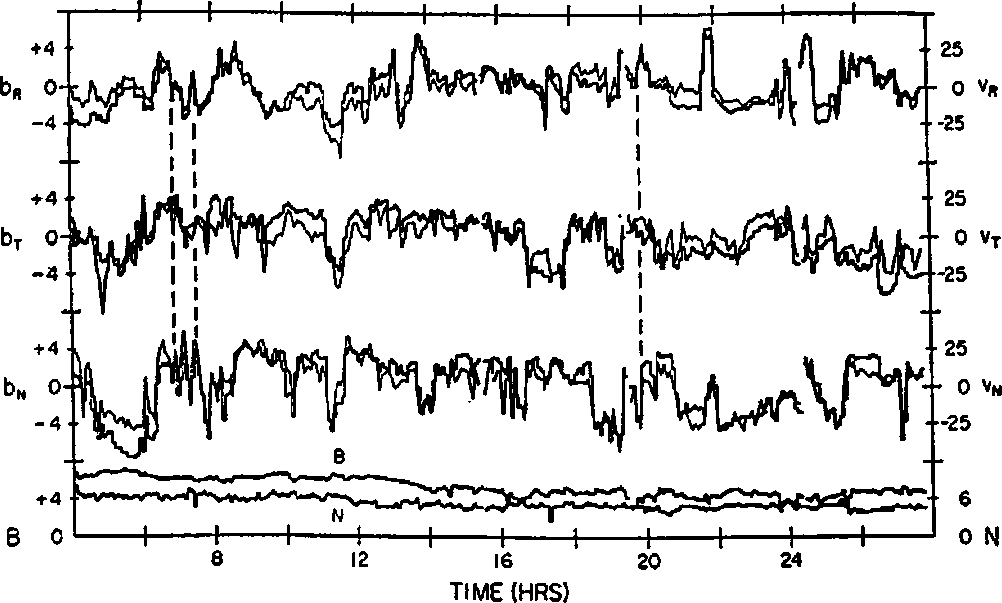
\includegraphics[width=0.8\columnwidth]{Fundamentos/fig3.png}
  \caption{Veintiocho horas de datos de plasma y de campo magnético,
    demostrando la presencia de ondas de Alfv\'en casi puras. Las seis
    curvas superiores corresponden a las componentes de las
    velocidades y del campo magnético, promediadas sobre el periodo de
    muestreo de la sonda. Los ejes verticales a la derecha
    corresponden a las componentes de la velocidad en km/seg ($R$ =
    radial, $T$ = tangencial, $N$ = normal, relativas al plano
    eclíptico); los ejes verticales a la izquierda corresponden a las
    componentes del campo magnético en nT. Las dos curvas inferiores
    corresponden a la fuerza del campo magnético y a la densidad
    numérica de protones (en cm$^{-3}$). Imagen extraída de
    \cite{belcher_large-amplitude_1971}.}
  \label{fig:equiparticion}
\end{figure}

Las simulaciones también tratan la cuestión del índice espectral en
MHD. Los espectros de energías obtenidos por las primeras simulaciones
computacionales de turbulencia MHD resultaron poco
concluyentes. Por ejemplo, simulaciones con resolución numérica de
$180^3$ puntos de grilla [\cite{politano_current_1995}] no pudieron
generar un rango inercial extendido. Simulaciones más recientes y con
mayor resolución [\cite{biskamp_scaling_2000}] proveyeron resultados
que apoyan la ley de Kolmogorov de los $-5/3$
(figura \ref{fig:normalizedspectrum}). El espectro mostrado en esta
figura ha sido multiplicado por $k^{5/3}$, resultando así en una
región plana que indica un claramente discernible, aunque pequeño,
rango inercial $\tilde{E}(\tilde{k})\tilde{k}^{5/3} =
\tilde{k}^{5/3}E_K/\left(\epsilon\eta^5\right)^{1/5} = \tilde{C}_K
F(\tilde{k})$, donde $\tilde{C}_K$ es una constante y
$\tilde{k}=kl_d$, con $l_d=\left(\mu^3/\epsilon\right)^{1/4}$ la
escala de disipación de Kolmogorov (asumiendo $\mu=\nu$).

\begin{figure}[h]
  \centering
  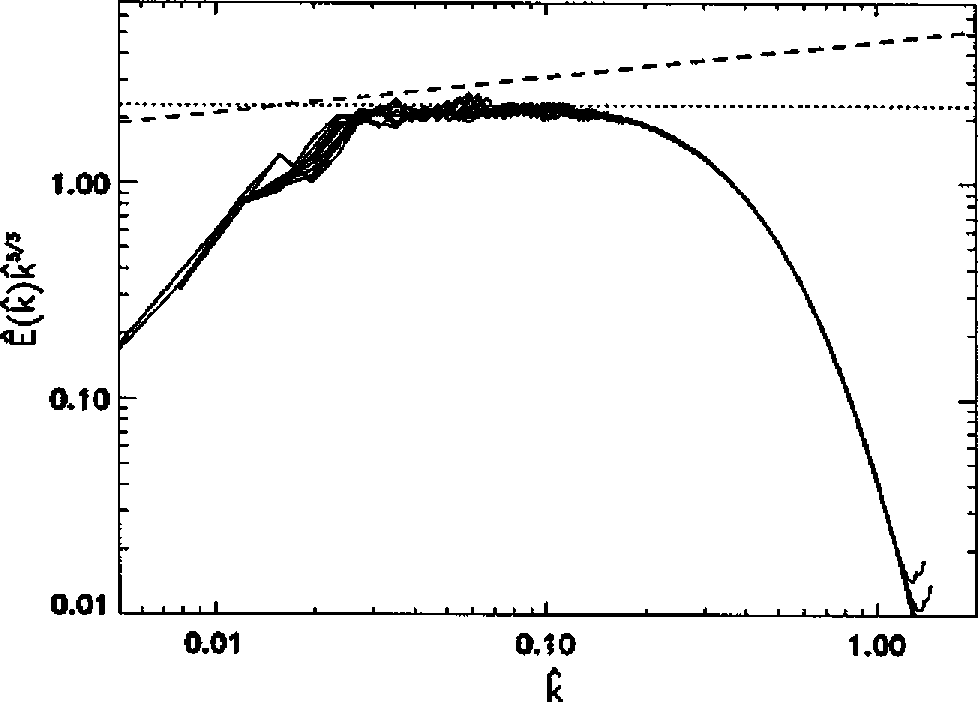
\includegraphics[width=0.8\columnwidth]{Fundamentos/fig4.png}
  \caption{Imagen del espectro normalizado, integrado angularmente,
    en turbulencia MHD versus $\hat{k} = k\ell_d$ (donde $\ell_d$ es
    la escala de disipación de Kolmogorov). Todas las curvas se
    encuentran multiplicadas por $k^{5/3}$. El escaleo de Kolmogorov
    se encuentra fuertemente sugerido por esta simulación numérica
    directa (curva sólida), con helicidad magnética nula. La línea
    discontinua indica el espectro $k^{-3/2}$ de Iroshnikov-Kraichnan
    (ver sección \ref{sec:escaleoI-K}), mientras que la línea punteada
    muestra el espectro de Kolmogorov, con $C_K = 2.3$. Imagen
    extraída de \cite{biskamp_scaling_2000}.}
  \label{fig:normalizedspectrum}
\end{figure}

Las hojas de corriente de pequeña escala son la característica
disipativa dominante en escalas pequeñas para turbulencia MHD, tanto
en tres dimensiones [\cite{biskamp_scaling_2000}] como en dos
[\cite{matthaeus_turbulent_1986}]. El rol crucial de la formación de
hojas de corriente y de reconexión debida a la turbulencia puede verse
[\cite{dmitruk_coronal_2002}] en modelos reducidos
\textit{wave-driven} de MHD que conceptualmente se encuentran entre el caso
puramente 2D y el puramente 3D. En 3D, las hojas de corriente están
mucho más distorsionadas, y encontrar los sitios de reconexión es más
difícil que en el caso 2D [\cite{politano_current_1995}]. La formación
de hojas de corriente asociadas con reconexión de estructuras
magnéticas cercanas es un aspecto fundamental de la turbulencia MHD,
que está relacionado con movimientos del tipo \textit{strain}.

La dinámica de las ondas de Alfvén, paralela al campo medio, no
controla la turbulencia, que en su lugar es gobernada por el
movimiento tipo \textit{eddies} perpendiculares al campo. Biskamp y
M\"uller argumentan que en tres dimensiones el movimiento arremolinado
puede dominar fácilmente la dinámica por sobre las ondas de Alfv\'en;
en consecuencia, el efecto de barrido por la propagación de ondas es
más débil que el \textit{straining} en turbulencia MHD 3D en ausencia
de un campo magnético DC. Esto indica que la transferencia de energía
local y las interacciones locales son dominantes.

\subsubsection{Cuando la propagación de Alfv\'en es dominante: escaleo de Iroshnikov-Kraichnan}\label{sec:escaleoI-K}

La forma más simple de incorporar efectos de la propagación de Alfv\'en
es asumir isotropía estadística, pero con la escala de tiempos de
descorrelación controlada por el periodo de una onda de Alfv\'en
característica.  De esta forma, \cite{iroshnikov_turbulence_1964} y
\cite{kraichnan_inertial-range_1965} retuvieron las suposiciones
básicas de Kolmogorov de isotropía y localidad en el número de onda de
las interacciones no lineales. Las fluctuaciones de pequeña escala son
vistas como paquetes de onda de Alfv\'en viajando junto al campo
magnético y sufriendo breves ``colisiones'' con los paquetes de onda
propagándose en sentido opuesto. Específicamente, Iroshnikov y
Kraichnan sugirieron que las correlaciones triples de velocidades en
turbulencia MHD decaen en un tiempo del orden del periodo de una onda
de Alfv\'en. Entonces, $\tau_T = \tau_A$, $\tau_A = (V_A k)^{-1}$, y
$\epsilon = \tilde{C}^2 \tau_T(k) k^4 E^2(k)$. Como resultado, se
obtiene el conocido espectro $k^{-3/2}$ de Iroshnikov-Kraichnan.

\cite{grappin_alfvenic_1982} examinaron las propiedades de la cascada de
Iroshnikov-Kraichnan utilizando la aproximación 3D de
\textit{EDQNM}. Encontraron, luego de varios \textit{eddy turnover
  times}, un estado cuasiestacionario que exhibe un rango inercial que
escala como $-3/2$, con correlación nula entre el campo magnético y el
de velocidades. Simulaciones numéricas directas de 2D ofrecen soporte
a dicho escaleo [\cite{biskamp_dynamics_1989, biskamp_geometric_1993,
  galtier_parametric_1999}]. Biskamp y M\"uller
[\cite{biskamp_scaling_2000}] señalaron que en 2D, los movimientos
arremolinados son débiles, tal como manifiesta el espectro energético
empinado en turbulencia hidrodinámica 2D. Por lo tanto, el
\textit{straining} aparece debilitado, y el efecto de propagación inducido
por ondas de Alfv\'en domina los efectos de descorrelación.



\subsubsection{Fenomenología extendida}

\cite{matthaeus_extended_1989, zhou_models_1990} desarrollaron un
marco en el cual ambas escalas temporales, $\tau_{nl}$ y $\tau_A$,
coexisten, de una forma análoga a la composición del tiempo de
correlación triple en la clausura \textit{EDQNM}
[\cite{pouquet_strong_1976}]. El punto es que el tiempo de vida de las
correlaciones de las transferencias $\tau_T(k)$ se calcula más
precisamente teniendo en cuenta las influencias de ambos agentes
externos y de las interacciones no lineales turbulentas. Componiendo
las tasas asociadas, obtenemos
\begin{equation}
  \frac{1}{\tau_T(\vec{k})} = \frac{1}{\tau_{nl}(\vec{k})} +
  \frac{1}{\tau_A(\vec{k})}.
\end{equation}
Notar que en general, pero dentro de la aproximación de transferencias
locales no lineales, el tiempo no lineal puede ser una función del
vector de onda $\vec{k}$. Esto se reduce a los casos límite esperados
cuando la fuerza del campo magnético efectivo tiende o bien a cero o
bien a infinito, por lo que $\tau_T$ se acerca a $\tau_{nl}$ o a
$\tau_A$, respectivamente. Acordemente, para el caso clásico de
turbulencia isotrópica, los espectros de energía, $E(k)\sim k^{-m}$,
tal como se muestra en la figura \ref{fig:Omnidirectional_vs_k}, tienen un exponente
de escaleo $3/2 \leq m \leq 5/3$, y se reduce a o bien la forma de
Iroshnikov-Kraichnan o bien la forma de Kolmogorov en los límites
apropiados.

\begin{figure}[h]
  \centering
  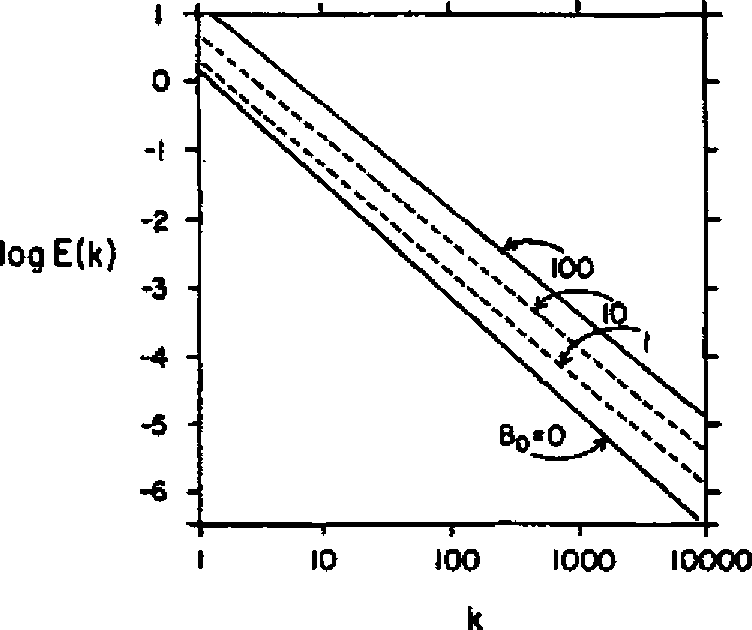
\includegraphics[width=0.7\columnwidth]{Fundamentos/fig7.png}
  \caption{Espectro energético omnidireccional versus número de onda,
    computado a partir de un espectro de energía generalizado. Se
    muestran cuatro valores de
    intensidad del campo magnético: $B_0 = 0$, $1$, $10$ y $100$. La
    pendiente se aplana y el nivel espectral se incremente a medida que
    la fuerza del campo aumenta, indicando una transición suave del
    escaleo $-5/3$ de Kolmogorov ($B_0 = 0$) a un escale a $B_0 = 100$
    que se acerca al $-3/2$ de Iroshnikov-Kraichnan. Extraída de
    \cite{matthaeus_extended_1989}.}
  \label{fig:Omnidirectional_vs_k}
\end{figure}



\subsection{MHD anisotrópico}
Kraichnan era consciente de que la presencia de un campo magnético de
gran escala que respalde la propagación de ondas de Alfv\'en puede
inducir una anisotropía [\cite{galtier_weak_2000}]. En el caso de
Iroshnikov-Kraichnan, el tiempo de Alfv\'en disminuye las
interacciones no lineales entre las fluctuaciones de Els\"asser
$z^\pm$, que aparecen simétricamente en la \cref{eq2:MHDElsasser}. Un
campo magnético de gran escala suprime el crecimiento de gradientes
paralelos al campo magnético, pero como los gradientes perpendiculares
no se ven afectados, los efectos no lineales (\textit{strain})
continúan bombeando energía hacia las escalas más pequeñas, sólo que
anisotrópicamente. Bajo ciertas circunstancias, esto lleva a estados
cuasi-bidimensionales.

Cuando la turbulencia es suficientemente bidimensional, la escala
temporal de Alfv\'en debida a propagaciones paralelas al
campo $B_0$ deja de ser pequeña en comparación con los tiempos de
interacción de \textit{strainings} intrínsecos de las fluctuaciones, y
la dinámica de $z^+$ y $z^-$ se vuelve similar a la turbulencia MHD
bidimensional, por lo que resulta casi independiente de $B_0$
[\cite{chen_inhibition_1997, hossain_phenomenology_1995}]. Esto
explica por qué las conclusiones principales de las simulaciones MHD
3D con un campo magnético externo impuesto
[\cite{oughton_influence_1994}], son consistentes con los estudios
bidimensionales [\cite{shebalin_anisotropy_1983}].

Entonces, es esperable que la estructura del espectro sea altamente
anisotrópica en la presencia de un campo DC, como fue originalmente
sugerido basándose en mediciones experimentales en el Culham Zeta
Device [\cite{robinson_structure_1971}]. El caso MHD bidimensional, el
cual no se ve afectado por la presencia de un campo DC perpendicular
fuerte, fue intensamente estudiado en la década del 70, y se sugirió
[\cite{fyfe_high-beta_1976, fyfe_dissipative_1977}] que el análisis de
Kolmogorov y su consiguiente escaleo de $-5/3$ sería aplicable al
rango inercial 2D asociado con una cascada de energía directa hacia
las escalas pequeñas. Este resultado estimuló el debate teórico, que
continuó durante más de 20 años.

A diferencia de caso 2D considerado por \cite{fyfe_dissipative_1977},
en el cual el campo DC define un plano perpendicular,
\cite{shebalin_anisotropy_1983} estudió MHD 2D en un plano que
contiene al campo DC. Esto define una dirección preferencial
adicional, y la anisotropía puede desarrollarse en el plano 2D. Las
simulaciones 2D incompresibles de \cite{shebalin_anisotropy_1983}
revelaron el desarrollo de una anisotropía fuerte y distintiva: la
energía se acumula preferencialmente en los vectores de onda $\vec{k}$
perpendiculares a $\vec{B}_0$. \cite{oughton_influence_1994} confirmó
los resultados de Shebalin en tres dimensiones encontrando que, con un
campo magnético DC, la transferencia de energía a modos
perpendiculares aumenta, comparativamente a los paralelos. Oughton
encontró que la anisotropía tiende a incrementarse con (i) la fuerza
del $B_0$ (con saturación a partir de $B_0 \geq 3b$); (ii) el número de
onda $k$; (iii) los números de Reynolds mecánico y magnético; (iv) el tiempo
(con saturación dependiendo el número de Reynolds), y (v)
el decrecimiento de la correlación cruzada.

La manifestación de anisotropía espectral en el espacio real es la
aparición de gradientes perpendiculares a la dirección media del campo
magnético, más intensos que los gradientes a lo largo del campo. Como
resultado, las longitudes de correlación son más largas a lo largo del
campo, y es esperable que las estructuras aparezcan elongadas en la
dirección de campo medio. Esta característica se encuentra ilustrada
en los resultados de las simulaciones numéricas de
la \cref{fig:currentdensity}.

\begin{figure}[h!]
  \centering
  \includegraphics[width=0.8\columnwidth]{Fundamentos/fig8.png}
  \caption{Mapas de color de la densidad de corriente $j_z$ en
    secciones transversales $x-y$ y $x-z$ de una simulación de
    turbulencia MHD 3D, con un campo magnético DC $B_0 \hat{z}$:
    arriba, $B_0 = 0$; al medio, $B_0/\delta B = 1$; abajo,
    $B_0/\delta B = 8$. Imagen extraída de
    \cite{zhou_colloquium_2004}}
  \label{fig:currentdensity}
\end{figure}


La anisotropía también es encontrada en la turbulencia del viento
solar. La evidencia para la anisotropía espectral del viento solar es,
hoy en día, indirecta; no obstante, ha ganado un peso considerable
por las indicaciones consistentes de anisotropía provenientes de
diferentes tipos de estudios [\cite{matthaeus_unquiet_1995}]. Las
observaciones directas sugieren que las fluctuaciones del viento solar
son anisótropas [\cite{carbone_model_1995}] y que contienen una mezcla
de excitaciones en vectores de onda casi perpendiculares
[\cite{bieber_dominant_1996}]. Adicionalmente, el rango inercial del
viento solar admite una distintiva varianza anisotrópica, con una
varianza paralela inhibida. En las simulaciones, la aparición de esta
característica requiere baja compresibilidad
[\cite{matthaeus_anisotropic_1996}].

Para ofrecer una interpretación simple y físicamente atractiva del
desarrollo de la anisotropía en la dirección perpendicular al campo
magnético DC aplicado, \cite{shebalin_anisotropy_1983} apela
a un argumento de interacción resonante de tres ondas. Esta
interpretación se basa en una teoría de turbulencia débil
[\cite{zakharov_kolmogorov_1992}], que sólo computa correciones de
primer orden a las soluciones de la ecuación lineal de MHD. En este
marco, los términos no lineales de las ecuaciones MHD cancelan
exactamente las soluciones de ondas, por lo que ondas propagándose en
la misma dirección no generan modos adicionales. Dos modos de Fourier
excitados pueden intercambiar energía eficientemente con un tercer
modo sólo si la tríada obedece la condición estándar de resonancia
[\cite{montgomery_anisotropic_1995}]: $\vec{k_1} + \vec{k_2} =
\vec{k_3}$, y $\omega(\vec{k_1}) - \omega(\vec{k_2}) = \pm
\omega(\vec{k_3})$. Aquí, $\vec{k_1}$ y $\vec{k_2}$ son vectores de
onda asociados a dos modos excitados de Fourier que están excitando
mediante resonancia un tercer vector de onda $\vec{k_3}$. En el límite
lineal, se asume que los tres modos tienen asociada una dependencia
temporal del tipo $\exp(-i\omega t)$, y satisfacen la relación
$\omega(\vec{k}) = \vec{k}\cdot\vec{V}_A$, donde $\vec{V}_A =
\vec{B}_0/(4\pi\rho)^{1/2}$ es el vector de velocidad de Alfv\'en
asociado al campo magnético medio. Las ondas interactuantes deben
propagarse en direcciones opuestas, que dan cuenta por el signo de
diferencia en el lado izquierdo de la condición para las
frecuencias. Las tríadas de ondas que satisfagan $\vec{k_1}\cdot
\vec{V}_A - \vec{k_2}\cdot \vec{V}_A = \pm \vec{k_3}\cdot \vec{V}_A$
tendrán acoplamiento no nulo sólo si $\vec{k_1}\cdot \vec{V}_A = 0$ ó
$\vec{k_2}\cdot \vec{V}_A = 0$. En consecuencia, $\vec{k_1}$ ó
$\vec{k_2}$ tendrán componente nula a lo largo de $\vec{B}_0$.

Las consecuencias físicas de los acoplamientos de tres ondas puedes
resumirse de la siguiente manera: al orden principal, no hay
transferencia para un campo magnético DC impuesto; la transferencia en
la dirección perpendicular no es impedida por el acoplamiento de ondas
de Alfv\'en que suprime la transferencia paralela; consecuentemente,
la transferencia MHD perpendicular se realiza de manera muy similar al
caso MHD 2D [\cite{fyfe_dissipative_1977}]. De esta manera, es esperable
un espectro $k_\perp^{-5/3}$ para los vectores de onda
perpendicular. En la dirección paralela, se produce una transferencia
débil, pero por cada paso en $k_\parallel$, mucha energía es desviada
a $k_\perp$ más grandes. En consecuencia, es esperable que el espectro
paralelo sea una exponencial $\sim \exp(-k_\parallel)$. La primera
sugerencia de esto la plantearon \cite{montgomery_density_1987}.

Aunque la justificación física para la ocurrencia de la anisotropía
espectral haya sido dada en el espacio de números de onda, es
esperable que este fenómeno tenga una manifestación en el espacio real
con algún grado de localidad. Un campo magnético de escala
suficientemente grande debería inducir efectos locales que sean
indistinguibles de un campo DC estrictamente uniforme. En
consecuencia, sería esperable poder entender la ocurrencia de
anisotropías enteramente en el contexto de un sistema teniendo
corrientes eléctricas localizadas y campos magnéticos con escala
estrictamente finita. Hay muchos estudios numéricos
[\cite{cho_anisotropy_2000, milano_local_2001}] que se encargan de
este problema, y concluyen que la anisotropía descripta posee
efectivamente un análogo puramente local. El punto básico vuelve a las
mediciones en el Culham Zeta Device de
[\cite{robinson_structure_1971}], que encontraron que la correlación
de las fluctuaciones magnéticas caen mucho más rápidamente en las
direcciones perpendiculares a un campo aplicado de gran escala, que
respecto de la dirección paralela. Aplicaciones de estas ideas a datos
simulados indican que la anisotropía efectivamente ocurre en forma
local. Las correlaciones caen más rápidamente en las direcciones
transversales al campo magnético medio calculado localmente. La
anisotropía resulta ser más grande a escalas pequeñas
[\cite{cho_anisotropy_2000}] y mayor donde la fuerza del campo medio
local es mayor.

%%% Mininni
\subsection{Localidad de las interacciones a partir de las transferencias \emph{shell-to-shell}}
En los últimos años, el aumento de la potencia de las computadoras ha
permitido la exploración numérica de turbulencia MHD en diferentes
regímenes. Además, los estudios de transferencia energética
\textit{shell-to-shell} [\cite{alexakis_shell_2005, dar_energy_2001,
  debliquy_energy_2005}] han permitido el cálculo explícito de las
interacciones de escala en la turbulencia de MHD utilizando el
resultado derivado de las simulaciones y sin la necesidad de calcular
las interacciones triádicas más complejas.

En líneas generales, las transferencias \textit{shell-to-shell}
$T_{uw}(Q, K)$ permiten analizar la transferencia energética
entre dos campos $\vec{u}$ y $\vec{w}$ (que pueden ser $\vec{v}$,
$\vec{b}$, $\vec{z^+}$ o $\vec{z^-}$), entre dos cascarones $Q$ y $K$
[\cite{mininni_scale_2011}].

Los resultados obtenidos indican, en todos los casos, que las
transferencias $T_{vv}$ y $T_{bb}$ tienen un comportamiento local: la
energía es transferida a escalas vecinas más pequeñas, de una forma
similar a la turbulencia hidrodinámica [\cite{alexakis_imprint_2005,
  mininni_large_2006}]. En cambio, $T_{vb}$ y $T_{bv}$, que expresan el
intercambio de energía entre los campos magnético y de velocidades,
han tenido comportamientos variados, dependiendo del problema
estudiado.

En el caso de turbulencia homogénea e isotrópica, con forzado sólo
mecánico, Alexakis, Mininni y Pouquet [\cite{alexakis_imprint_2005}]
encontraron una pequeña pero no despreciable transferencia no
local. Los resultados pueden observarse en la
\cref{fig:transferfunctions}. En dicha figura se puede observar las
funciones de transferencia típicas del caso. Se puede ver que tanto
$T_{vv}$ como $T_{bb}$ son locales, con un pico negativo para $K<Q$ y
uno positivo para $K>Q$, que indica que la energía es removida de las
escalas con números de onda vecinos más chicos y transferida hacia los
estados con números de onda vecinos más grandes. También se puede
observar que para $T_{vb}$ (transferencia de energía mecánica a
magnética) el comportamiento es distinto. En este caso, el flujo a
gran escala inyecta energía (a través del \textit{straining})
directamente en el campo magnético a todas las escalas. Esto se
manifiesta como un pico en la escala de fuerza mecánica para todos los
valores de $Q$, y como una meseta positiva que se extiende hasta
$K\approx Q$.  En otras palabras, en una capa $K$ dada, el campo
magnético recibe energía del campo de velocidad en todas las capas con
$Q<K$, y da energía al campo de velocidad en las capas con $Q>K$. Este
resultado se puede interpretar como sustento del campo magnético
contra la disipación Óhmica por acción de un dínamo: para mantener el
campo magnético cuando sólo se excita el campo de velocidad, es
necesario un flujo no nulo de energía desde el campo de velocidad
hacia el campo magnético, en todo momento. No obstante, cabe señalar
que a pesar de la importancia que cumple este efecto, en el estado
estacionario esta transferencia no local es pequeña en comparación con
las transferencias locales, representando alrededor de un $10\%$ ó
$20\%$ en las resoluciones estudiadas [\cite{mininni_large_2006}]. Al
considerar las variables de Els\"asser, se observó que las funciones
de transferencia se volvían más locales aún.
\begin{figure}[h!]
  \centering
  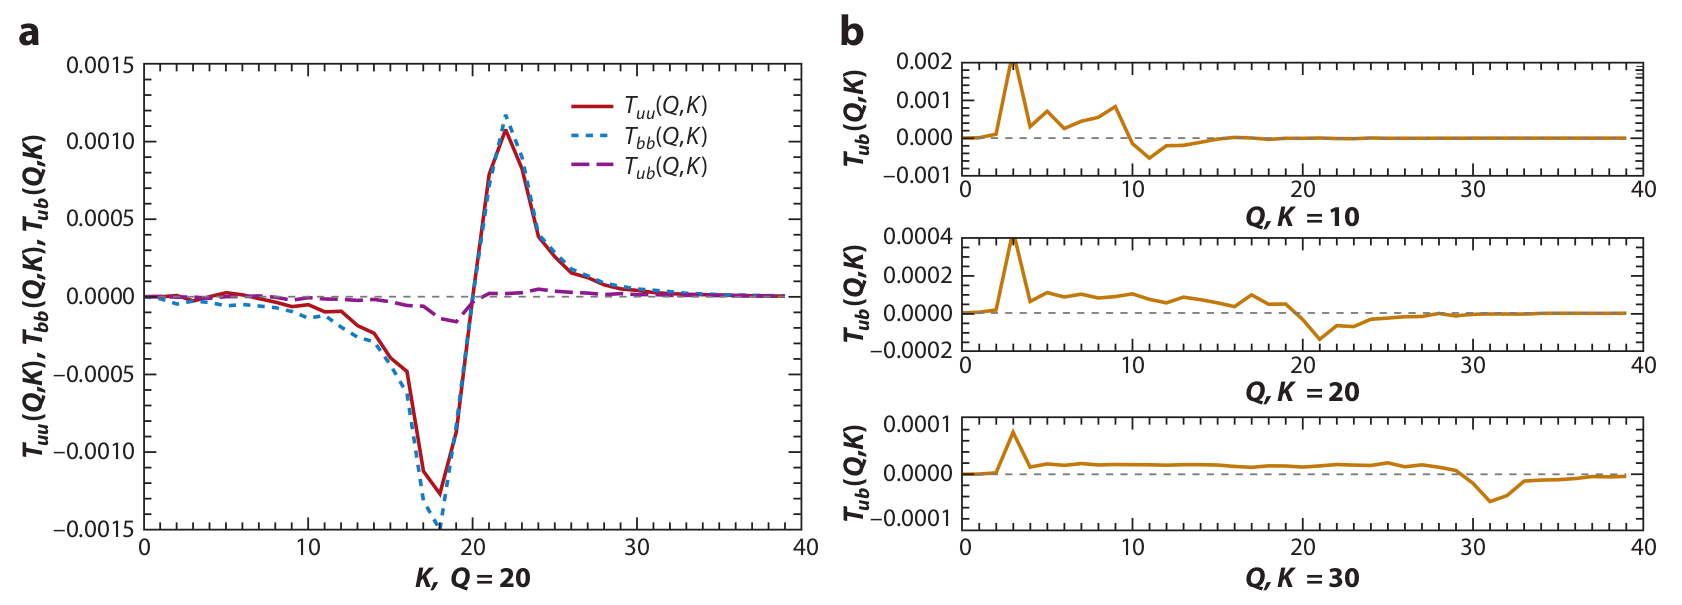
\includegraphics[width=0.99\columnwidth]{Fundamentos/figtransferfunctions.png}
  \caption{(a) Funciones de transferencia para turbulencia MHD forzada
    mecánicamente, para el cascarón $Q = 20$. Las funciones $T_{vv}$ y
    $T_{bb}$ son locales, con un pico negativo para $K<Q$ y uno
    positivo para $K>Q$, que indica que la energía es removida de los
    números de onda vecinos más chicos y transferida hacia los números
    de onda vecinos más grandes. La transferencia energética desde el
    campo magnético al cinético es mucho más pequeña en amplitud, y
    también resulta local. (b) Función de transferencia $T_{vb}$
    (mecánica a magnética), para distintos valores de $K$. Esta
    función es no local, con un pico alto en la escala del forzado y
    con un \emph{plateau} constante y positivo que se extiende hasta
    $K\approx Q$. Figura adaptada de \cite{alexakis_imprint_2005}.}
  \label{fig:transferfunctions}
\end{figure}


Otro caso estudiado corresponde al decaimiento turbulento libre, donde
los efectos no locales son despreciables
[\cite{debliquy_energy_2005}]. Es este caso, tanto $T_{vv}$ y $T_{bb}$,
como $T_{vb}$ y $T_{bv}$, resultan locales y de transferencia de
grandes escalas a pequeñas. Se obtuvieron resultados similares en
observaciones del viento solar [\cite{bruno_solar_2005}]. Las
diferencias entre los casos de decaimiento forzado y libre pueden
entenderse al notar que, en los recorridos forzados mecánicamente, el
campo de velocidad debe suministrar energía continuamente al campo
magnético para sostenerlo contra la disipación Óhmica. Este no es
necesariamente el caso de las corridas en decaimiento libre, en las
que ambos campos se disipan en el tiempo.

Por último, el caso anisotrópico resulta más complejo. Por lo pronto,
no resulta tan evidente cómo tomar las distintas capas. Una
posibilidad es introducir funciones de transferencia
\textit{shell-to-shell} tomando como capas secciones cilíndricas
(asociados con el número de onda $k_\perp$ perpendicular al campo
magnético medio) y secciones planas (asociadas a los
$k_\parallel$). Las funciones de transferencia para las energías de
Els\"asser fueron locales en las dos direcciones, independientemente
de la amplitud del campo magnético externo. Sin embargo, las
interacciones entre las ondas de Alfv\'en contrapropagantes resultaron
ser no locales. Para campos magnéticos fuertes, la mayor parte del
flujo de energía en la dirección perpendicular fue resultado de
interacciones con modos con $k_\parallel = 0$
(\cref{fig:mininnianisotropo}). Sin embargo, en la dirección paralela,
los modos $k_\parallel = 0$ no pueden transferir energía, y se observó
que la mayoría de las interacciones tienen lugar con modos cercanos a
$k \approx 0$. Los resultados están en acuerdo cualitativo con las
predicciones de la teoría de la turbulencia débil
[\cite{galtier_weak_2000}] y con algunos modelos fenomenológicos no
locales [\cite{alexakis_nonlocal_2007}].
\begin{figure}[h!]
  \centering
  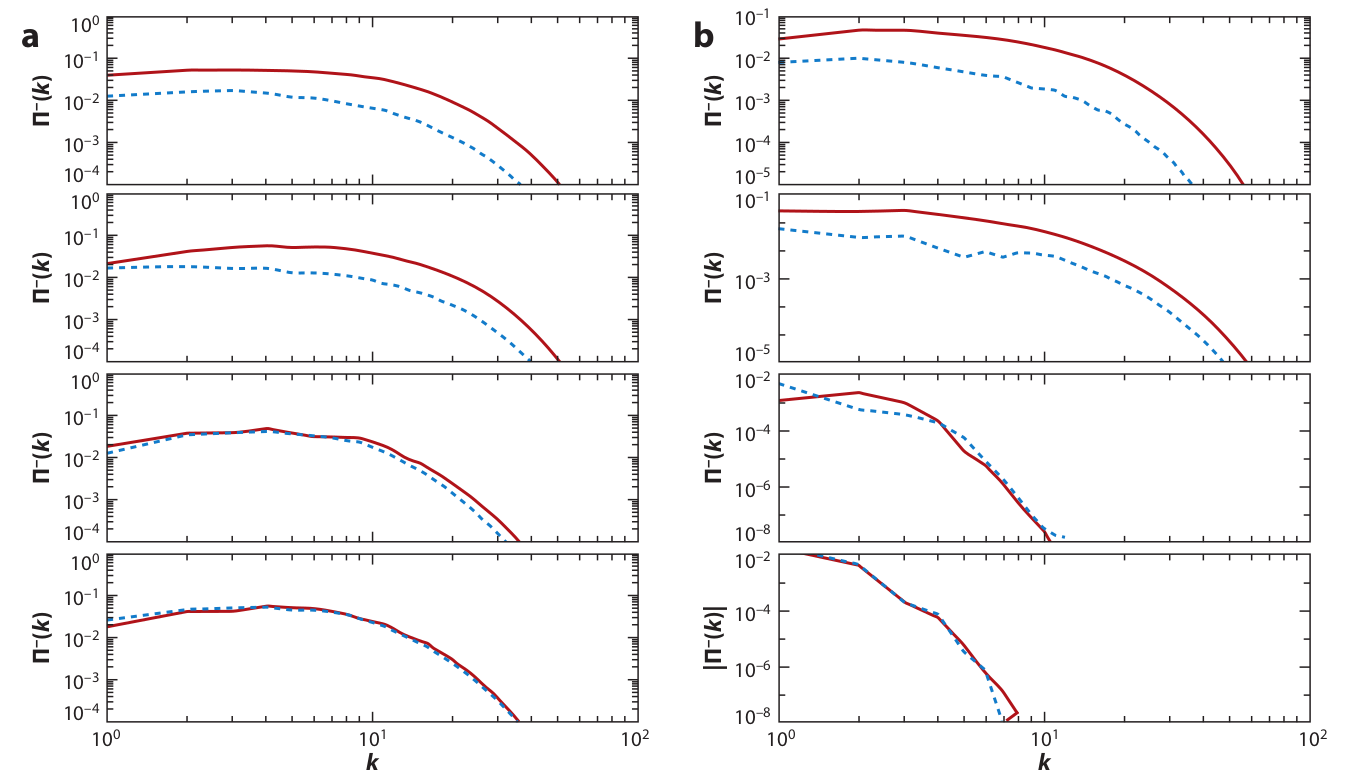
\includegraphics[width=0.99\columnwidth]{Fundamentos/figmininnianisotropo.png}
  \caption{(a) Flujo de energía total (líneas rojas continuas) a
    través de cilindros y flujo parcial asociado con interacciones con
    modos con $k_\parallel = 0$ (líneas azules discontinuas), con
    cuatro valores diferentes del campo magnético externo $B_0$, desde
    $0$ hasta $15$ (desde arriba hacia abajo). (b) Igual que en el
    panel \emph{a}, pero con el flujo total y el flujo parcial
    asociados con interacciones con modos con $k_\parallel = 1$ a
    través de planos. Figura adaptada de
    \cite{alexakis_anisotropic_2007}.}
  \label{fig:mininnianisotropo}
\end{figure}

Las consideraciones anteriores llevaron a varios autores a considerar
si algunos de los supuestos habituales en la turbulencia hidrodinámica
se mantenían efectivamente en el caso de MHD. A partir de análisis de
la transferencia de capa a capa, el escenario más realista para la
energía está representado en la \cref{fig:transferfunctionsMHD}: las
interacciones entre los mismos campos son en su mayoría locales, y las
interacciones entre la velocidad y el campo magnético pueden tener
diferentes grados de no localidad dependiendo de si la turbulencia es
forzada o decae libremente, dependiendo de cómo se mantengan la
velocidad y los campos magnéticos contra la disipación en el caso
forzado, y dependiendo de la presencia de un campo magnético
externo. Actualmente no está claro si el grado variable de no
localidad con la configuración convergerá a una solución universal
para números de Reynolds muy grandes.
\begin{figure}[h!]
  \centering
  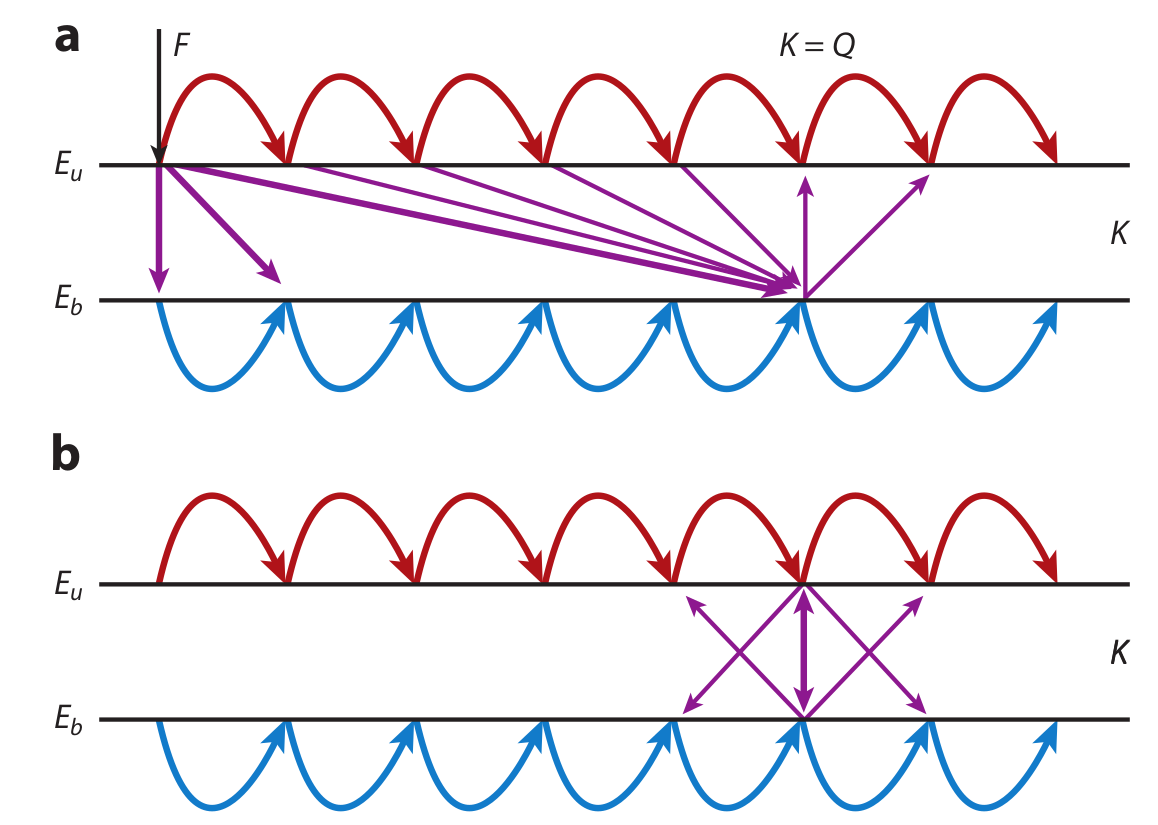
\includegraphics[width=0.8\columnwidth]{Fundamentos/figtransferfunctionsMHD.png}
  \caption{Diagrama de las diversas transferencias de energía
    \emph{shell-to-shell} identificadas en simulaciones de turbulencia
    MHD isotrópica y homogénea. Las transferencias de $T_{vv}$ se
    muestran en rojo, las transferencias de $T_{bb}$ en azul y las de
    $T_{vb}$ y $T_{bv}$ en violeta. El grosor de las flechas indica
    aproximadamente la fuerza de las transferencias. (a) Simulaciones
    forzadas mecánicamente. En la capa $K$, el campo magnético recibe
    energía del campo de velocidad en todas las escalas más grandes y
    le da energía al campo de velocidad en escalas ligeramente más
    pequeñas. (b) Turbulencia en decaimiento libre. $T_{vb}$ y
    $T_{bv}$ transfieren energía sólo localmente. En ambos casos, las
    transferencias $T_{vv}$ y $T_{bb}$ son locales y dan la mayor
    contribución al flujo.}
  \label{fig:transferfunctionsMHD}
\end{figure}

En cualquier caso, existe un consenso cada vez mayor de que la
turbulencia de MHD es menos local que la turbulencia hidrodinámica,
aunque no es claro en qué medida. Por el momento, no está claro si
estos efectos desaparecerán para un mayor número de Reynolds; tampoco
está claro, en caso de permanecer, qué impacto tendrán en la dinámica
del flujo y en qué condiciones. Sin embargo, los diferentes grados de
no localidad observados en las resoluciones actuales, y la existencia
de procesos no locales en MHD (como, por ejemplo, el dínamo a pequeña
escala), requieren una discusión sobre la validez de la hipótesis de
localidad de interacciones, y si existe un solo tipo de turbulencia
MHD o muchos. Estos son puntos a tener en cuenta al realizar un
análisis fenomenológico o teórico. Además, esta coexistencia de
interacciones locales y no locales con el modo con $k=0$ confirman el
análisis temporal anterior: se encuentran presentes
el \textit{straining}, el \textit{sweeping} aleatorio y las
interacciones Alfv\'enicas con $B_0$.

%%% END Mininni



\subsection{Comentarios de los espectros de frecuencias}\label{sec2:SpectraFreq}

En la década de 1970, la investigación de la turbulencia hidrodinámica
se dirigió al estudio del tiempo de descorrelación del campo de
velocidades [\cite{tennekes_eulerian_1975, orszag_numerical_1972,
orszag_analytical_1970, comte-bellot_simple_1971}]. Además de las
correlaciones espaciales, también cobró interés el estudio del
espectro en frecuencias (correlaciones de dos tiempos y un punto
espacial) más allá de la hipótesis de ``turbulencia congelada''. Si
bien el espectro Euleriano en frecuencias resulta un tanto
controversial en algunos casos particulares [\cite{chen_sweeping_1989,
nelkin_time_1990}], la conclusión principal fue que el
\textit{sweeping} aleatorio domina la descorrelación temporal en el rango
inercial para el caso hidrodinámico
[\cite{zhou_non-gaussian_1993,sanada_random_1992}].

Nuevamente, el caso MHD resulta mucho más complejo, quedando aún
muchas preguntas acerca de cuál es la escala temporal dominante de la
descorrelación temporal [\cite{busse_2010_lagrangian}].
Recientemente, \cite{servidio_time_2011} realizaron un estudio para
analizar la descorrelación temporal para el caso de turbulencia MHD
isotrópica. El resultado principal que obtuvieron fue que, como en
hidrodinámica, la descorrelación temporal en MHD es gobernada por
interacciones no locales (en este caso, \emph{sweeping} aleatorio y
propagación de Alfv\'en), tal como puede apreciarse en
la \cref{fig2:ServidioDescorrelacion}. Sin embargo, no pudieron
distinguir entre los efectos del \emph{sweeping} y de la distorsión
Alfv\'enica. En el capítulo \ref{ch:P1} ahondaremos este punto.
\begin{figure}[h]
  \centering
  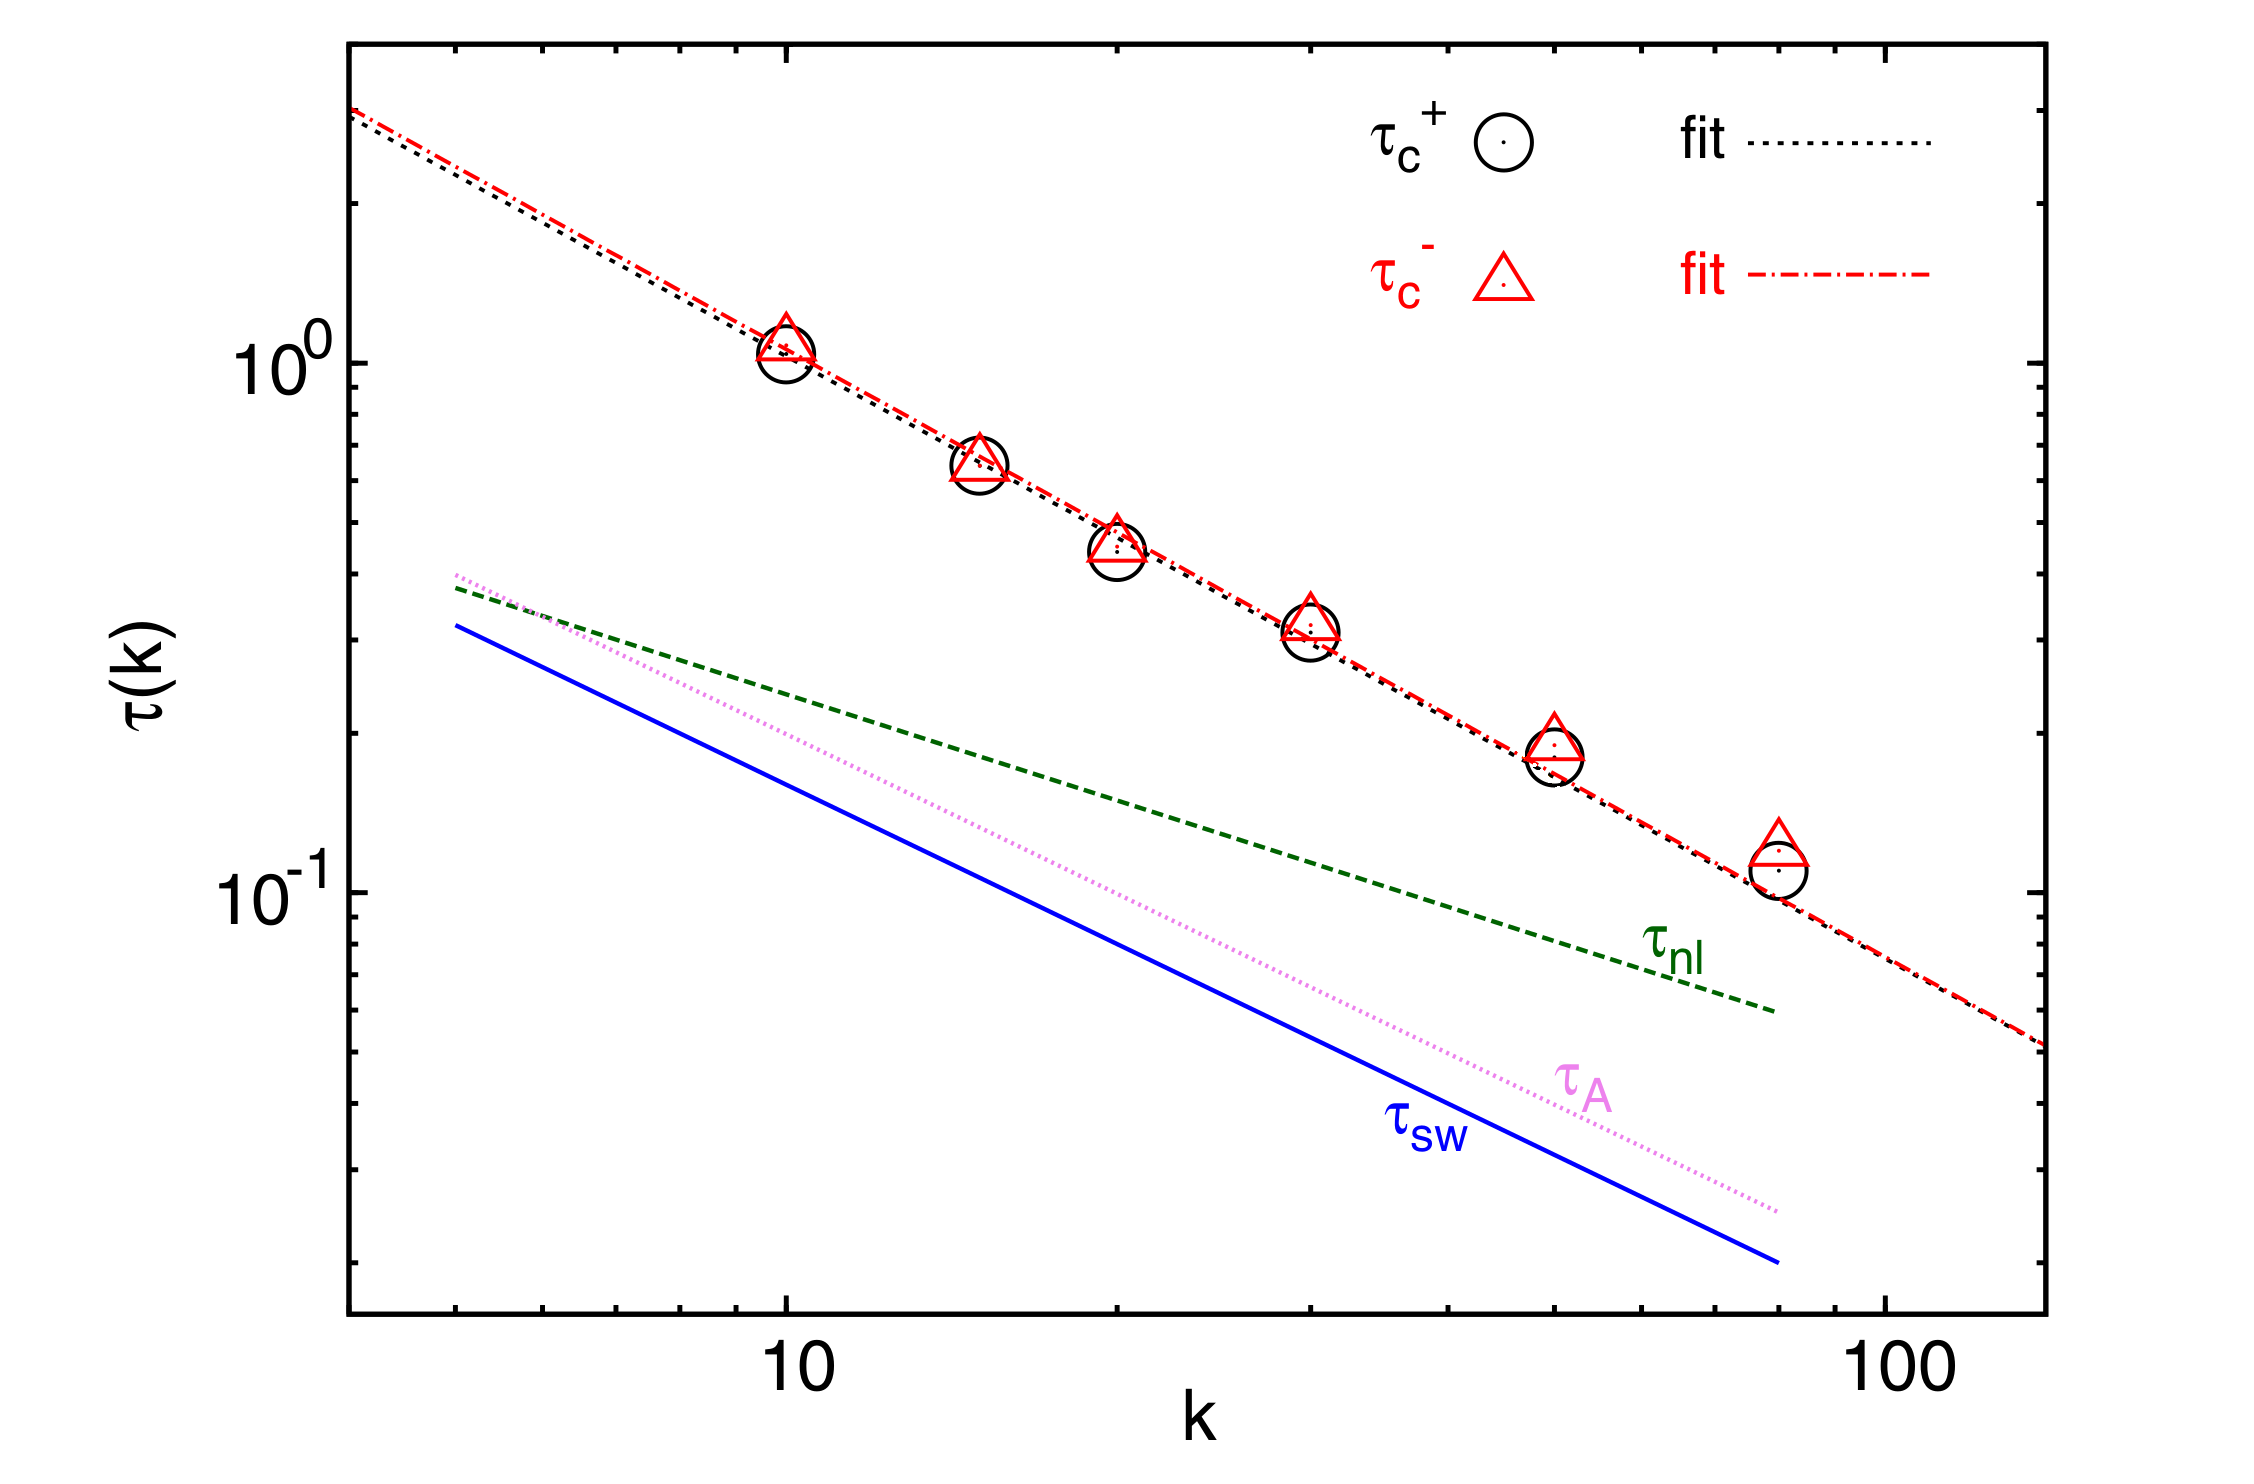
\includegraphics[width=0.8\columnwidth]{Fundamentos/ServidioDescorrelacion.png}
  \caption{Tiempos de descorrelación $\tau_C^\pm$ (círculos negros y triángulos rojos) en función del número de onda $k$ para el caso MHD isótropo. Se muestran los distintos tiempos característicos: no lineal ($\tau_{nl}$, línea discontinua verde); de Alfv\'en ($\tau_{A}$, línea punteada rosa), y de \emph{sweeping} aleatorio ($\tau_{A}$, línea azul). Se observa claramente cómo los tiempos de descorrelación escalean como $\tau_{A}$ y como $\tau_{sw}$. Imagen adaptada de \cite{servidio_time_2011}.}
  \label{fig2:ServidioDescorrelacion}
\end{figure}





\section{Discusión y conclusiones}\label{sec:FundConclusiones}

Con la base de las propiedades física discutidas, es posible
desarrollar una metodología para estimar los espectros de energía y
las funciones de correlación en varios regímenes de turbulencia
MHD. La idea es la siguiente: se estima una escala de tiempo del
espectro de transferencia, incorporando efectos debidos tanto a los
movimientos no lineales de \textit{straining} como a la influencia
de barrido por la propagación de ondas. La influencia
relativa de estos efectos será relacionada con el grado y el tipo de
anisotropía esperada; por ejemplo, si la anisotropía se debe a un
campo magnético DC externo fuerte o si se debe a campo magnético
local. Acordemente, la transferencia espectral es o bien isótropa,
cuando se toman en consideración grandes muestras de plasma, o bien es
anisótropa, cuando hay un campo magnético fuerte en las escalas
grandes. Con esta base, podemos examinar la tasa estacionaria de
transferencia de energía fenomenológicamente, haciendo uso de la
afirmación
\begin{equation}
  \epsilon = \Pi(k) = \tau_T(k) \frac{kE(k)}{\tau_{nl}^2},
\end{equation}
que no es más que la \cref{eq2:TR_sw}. En esta ecuación se
relacionan varios elementos físicos de la MHD:
\begin{itemize}
\item La transferencia de energía debe ser proporcional al tiempo de
  vida de la correlación triple, como en la \cref{eq2:transferRate}.
\item La fuerza de las interacciones no lineales es medida por el
  \textit{eddy turnover} o la escala temporal no lineal, como en
  la \cref{eq2:tauNL}.
\item Finalmente, el flujo espectral de energía debe ser definido de
  una forma (\cref{eq2:TR_sw}) que sea compatible con los ítems
  anteriores. Esta es más que una relación formal, y de hecho puede
  ser utilizada para hacer estimaciones de la forma del espectro en
  una variedad de casos físicos interesantes.
\end{itemize}

Este procedimiento nos permite fácilmente entender la física de las
teorías de Kolmogorov y de Iroshnikov-Kraichnan, así como sus
diferencias. Además, no se requieren teorías de clausura complejas o
esquemas de perturbaciones. Si, adicionalmente, queremos desarrollar
aproximaciones para las funciones de correlación tiempo-dependientes,
como las funciones de correlación Eulerianas (un punto espacial, dos
temporales), o las descorrelaciones de dos tiempos que aparecen en las
teorías de clausura, deberíamos proceder de una manera análoga:
adoptamos una forma funcional razonable para la función de correlación
temporal, dependiente de una única escala temporal, digamos,
del mismo tiempo de transferencia espectral.

En este capítulo hemos intentado dar un panorama del rol influyente de
distintas escalas temporales para establecer la transferencia de
energía, las cascadas, la no localidad y la anisotropía, en
turbulencia MHD. Como en el caso hidrodinámico, la escala temporal
``nativa'' puede dividirse en movimientos de \textit{straining}
debidos a la propia distorsión de los \textit{eddies}, y a movimientos
tipo de barrido (ya sea por el propio \textit{sweeping} aleatorio o
por la propagación de ondas) que desplazan estructuras de pequeña
escala bajo la influencia de los campos de gran escala. En MHD los
movimientos de \textit{straining} son dominantemente locales en
escala, dado que las distorsiones no lineales son más efectivas para
interacciones entre \textit{eddies} de aproximadamente el mismo
tamaño. No obstante, las interacciones no locales son más
complejos que en hidrodinámica debido al efecto de propagación de
Alfv\'en. El barrido debido a propagación de ondas Alfv\'enicas
introduce un nuevo nivel de no-localidad en MHD y una fuerte tendencia
a que la transferencia espectral ocurra anisotrópicamente respecto de
la dirección del campo magnético.

En el pasado se han hecho muchas diferencias entre los espectros de
Kolmogorov y de Iroshnikov-Kraichnan, y ambas posibilidades suelen ser
comparadas en simulaciones y en observaciones interplanetarias, con el
aparente objetivo de plantear una distinción firme entre estas
posibilidades. Sin embargo, variando la escala temporal para el
decaimiento de las funciones de correlación de transferencia, se ve
que en turbulencia MHD hay una variación suave entre esos límites.
%% La
%% observación de varios índices espectrales en varios casos es un
%% indicativo del aumento de los efectos de \textit{sweeping} respecto de
%% los efectos de \textit{straining}, o de los efectos locales respecto
%% de los no locales, de acuerdo a cómo las condiciones prevalecientes
%% impacten en la relevancia de las escalas temporales.
%% La anisotropía es
%% controlada por variación del tiempo de descorrelación Alfv\'enico en
%% comparación a la escala temporal local no-lineal.
Esto abre a un
amplio rango de posibilidades para el espectro anisotrópico y para los
índices espectrales que puede aparecer en MHD.

Como discutimos, se espera un empalme suave entre Kolmogorov e
Iroshnikov-Kraichnan en el caso de turbulencia MHD isotrópico, al
cambiar el cociente entre el tiempo de Alfv\'en y el tiempo
no-lineal. La proporción es también dependiente del número de onda, y
la descorrelación más tipo ondular suele ocurrir a escalas más
pequeñas. Con un campo magnético uniforme fuerte, el espectro
energético anisotrópico resultante puede reducirse a $k_\perp^{-5/3}$
cuando las interacciones resonantes y el \textit{strain}
cuasi-bidimensional es el efecto de descorrelación dominante, o a
$k_\perp^{-3/2}$ cuando la descorrelación Alfv\'enica cuasi-2D de gran
escala es fuerte. Cuando los efectos cuasi-2D son débiles, el espectro
puede convertirse tanto en $k_\perp^{-2}$ (turbulencia ``débil''),
cuando las interacciones locales son dominantes, o en $k_\perp^{-3}$,
cuando las interacciones no locales son dominantes. Cuando tanto las
interacciones locales como las no locales están presentes, el espectro
varía suavemente entre estos límites.

Consideraciones similares de las escalas temporales nos permiten
acercarnos a un modelado de las funciones de correlación Eulerianas
que aparecen en MHD. En este caso, como hemos mencionado,
el \textit{sweeping} aleatorio se torna, junto a la propagación
Alfv\'enica, uno de los efectos preponderantes. En los próximos capítulos
analizaremos la influencia de cada uno de estos efectos en los espectros
espacio-temporales y en las funciones de correlación, lo que nos permitirá
distinguir cuál es el dominante en las distintas situaciones.

%% Debe hacerse notar que la evidencia tanto observacional como de
%% simulaciones sólo ha identificado y analizado algunos de los regímenes
%% MHD que se han discutido, y es necesario estudiar más exhaustivamente
%% los regímenes de los parámetros MHD, incluyendo un amplio rango del
%% número de Reynolds, helicidad cruzada, anisotropía muy fuerte,
%% transición entre transferencia espectral local y no local, MHD que se
%% aleja considerablemente de equipartición entre energías cinética y
%% magnética, y la influencia de varios posibles efectos de disipación
%% cinética. La disponibilidad de varias escalas temporales hace que la
%% turbulencia MHD sea más compleja y multifacética que su contraparte
%% hidrodinámica, haciendo que probablemente permanezca como un área de
%% estudio activa.
